\documentclass[12pt]{article}

%Graphic packages
\PassOptionsToPackage{dvipsnames}{xcolor}
\usepackage{graphicx}
\usepackage{subcaption}
\graphicspath{ {../Images} }
\usepackage{tikz}
\counterwithin{figure}{subsection}

%References libraries
\usepackage{hyperref}
\usepackage[super]{natbib}
\newcommand{\textcite}[1]{\citeauthor{#1}~\citeyear{#1}}

%Format
\usepackage{placeins}
\usepackage{geometry}
\geometry{includeheadfoot,a4paper, textwidth=0.87\paperwidth, textheight=0.9\paperheight, headsep =30pt}
\usepackage[onehalfspacing]{setspace}
\usepackage{fancyhdr}
\pagestyle{fancy}
\renewcommand{\headrulewidth}{1.5pt}
\lhead{
\includegraphics[scale=0.05]{SB.png}}
\rhead{
\includegraphics[scale=0.1]{IDL.png}}
\chead{Docking methods}
\usepackage{multicol}
\usepackage{tocbasic}
\DeclareTOCStyleEntry[dynnumwidth]{tocline}{figure}

%Cover page
\newcommand{\CoverPage}{
	\noindent
	\fbox{
		\noindent
		\begin{minipage}[c]{0.87\paperwidth}
			\begin{center}
				\vspace{2cm}
				{\huge\textbf{Synthetic Biobots}}\\
				\vspace{3cm}
				{\Huge\textbf{Docking Methods}}\\
				\vspace{3cm}
				
\includegraphics[scale = 0.3]{SB.png}\\
				\vspace{2cm}
				{\Large
					\textbf{Author:} Gerardo Cendejas-Mendoza\\\vspace{1cm}
					iGEM Design League\\\vspace{1cm}
					Season 2022
				}\vspace{2.5cm}
			\end{center}
		\end{minipage}
	}
}

%Chemistry packages
\usepackage{mol2chemfig}
\usepackage{chemfig}
\usepackage{caption}
\usepackage{chemmacros}
%\setchemfig{scheme debug=true}

% Arrow
% allow for editing Chemfig 
\catcode`\_=11

% Initial arguments:
% #1, #2: Same as for -U> (above arrow)
% #3: Additional label at midpoint (also above arrow)
% #4, #5, #6: Like #1, #2, and #3, but below arrow
% #7: Optional shift, default 0
% #8: Optional arrow radius
% #9: Optional arrow angle   
\definearrow9{-X>}{%
	\CF_arrowshiftnodes{#7}%
	\expandafter\draw\expandafter[\CF_arrowcurrentstyle](\CF_arrowstartnode)--(\CF_arrowendnode)node[midway](Xarrowarctangent){};%
	\CF_ifempty{#8}
	{\def\CF_Xarrowradius{0.333}}
	{\def\CF_Xarrowradius{#8}}%
	\CF_ifempty{#9}%
	{\def\CF_Xarrowabsangle{60}}
	{\pgfmathsetmacro\CF_Xarrowabsangle{abs(#9)}}
	% Draw top arrow (start)
	\edef\CF_tmpstr{[\CF_ifempty{#1}{draw=none}{\unexpanded\expandafter{\CF_arrowcurrentstyle}},-]}%
	\expandafter\draw\CF_tmpstr (Xarrowarctangent)%
	arc[radius=\CF_compoundsep*\CF_currentarrowlength*\CF_Xarrowradius,start angle=\CF_arrowcurrentangle-90,delta angle=-\CF_Xarrowabsangle]node(Xarrow1start){};
	% Draw bottom arrow (end)
	\edef\CF_tmpstr{[\CF_ifempty{#2}{draw=none}{\unexpanded\expandafter{\CF_arrowcurrentstyle}},-CF]}%
	\expandafter\draw\CF_tmpstr (Xarrowarctangent)%
	arc[radius=\CF_compoundsep*\CF_currentarrowlength*\CF_Xarrowradius,%
	start angle=\CF_arrowcurrentangle-90,%
	delta angle=\CF_Xarrowabsangle]%
	node(Xarrow1end){};
	% Draw bottom arrow (start)
	\edef\CF_tmpstr{[\CF_ifempty{#4}{draw=none}{\unexpanded\expandafter{\CF_arrowcurrentstyle}},-]}%
	\expandafter\draw\CF_tmpstr (Xarrowarctangent)%
	arc[radius=\CF_compoundsep*\CF_currentarrowlength*\CF_Xarrowradius,start angle=\CF_arrowcurrentangle+90,delta angle=\CF_Xarrowabsangle]node(Xarrow2start){};
	% Draw bottom arrow (end)
	\edef\CF_tmpstr{[\CF_ifempty{#5}{draw=none}{\unexpanded\expandafter{\CF_arrowcurrentstyle}},-CF]}%
	\expandafter\draw\CF_tmpstr (Xarrowarctangent)%
	arc[radius=\CF_compoundsep*\CF_currentarrowlength*\CF_Xarrowradius,%
	start angle=\CF_arrowcurrentangle+90,%
	delta angle=-\CF_Xarrowabsangle]%
	node(Xarrow2end){};
	% Insert labels
	\pgfmathsetmacro\CF_tmpstra{\CF_Xarrowradius*cos(\CF_arrowcurrentangle)<0?"-":"+"}%
	\pgfmathsetmacro\CF_tmpstrb{\CF_Xarrowradius*cos(\CF_arrowcurrentangle)<0?"+":"-"}%
	\ifdim\CF_Xarrowradius pt>0 pt
	\CF_arrowdisplaylabel{#1}{0}\CF_tmpstra{Xarrow1start}{#2}{1}\CF_tmpstra{Xarrow1end}%
	\CF_arrowdisplaylabel{#4}{0}\CF_tmpstrb{Xarrow2start}{#5}{1}\CF_tmpstrb{Xarrow2end}%
	\CF_arrowdisplaylabel{#3}{0.5}\CF_tmpstra\CF_arrowstartnode{}{}{}\CF_arrowendnode%
	\CF_arrowdisplaylabel{#6}{0.5}\CF_tmpstrb\CF_arrowstartnode{}{}{}\CF_arrowendnode%
	\else
	\CF_arrowdisplaylabel{#2}{0}\CF_tmpstra{Xarrow1start}{#1}{1}\CF_tmpstra{Xarrow1end}%
	\CF_arrowdisplaylabel{#5}{0}\CF_tmpstrb{Xarrow2start}{#4}{1}\CF_tmpstrb{Xarrow2end}%
	\CF_arrowdisplaylabel{#3}{0.5}\CF_tmpstra\CF_arrowstartnode{}{}{}\CF_arrowendnode%
	\CF_arrowdisplaylabel{#6}{0.5}\CF_tmpstrb\CF_arrowstartnode{}{}{}\CF_arrowendnode%
	\fi
}
% stop editting chemfig
\catcode`\_=8

%Math and table packages
\usepackage{amssymb}
\usepackage{multicol}
\usepackage{multirow}
\usepackage{booktabs}
\usepackage[para,online,flushleft]{threeparttable}
\usepackage{wrapfig}

%Color packages
\definecolor{MyBlue}{RGB}{39,193,227}

%\usepackage{lmodern}
%\usepackage[T1]{fontenc}
%\usepackage{anyfontsize}
%\newcommand\chemsize{\fontsize{5pt}{6pt}\selectfont}

\setcounter{secnumdepth}{3}

\begin{document}
	\setlength{\headsep}{20pt}
	\thispagestyle{empty}
	\CoverPage
	
	\newpage
	\setlength{\headsep}{30pt}
	
	\phantomsection
	\addcontentsline{toc}{section}{Introduction}
	\section*{Introduction}
	
	In this document is shown the docking methodology followed by the team  Synthetic Biobots during the iGEM Design League 2022 season. Molecular docking is a process to couple proteins with their ligands; for this project molecular docking was performed in order to support the decision of using the proteins that were selected as part of the biosynthetic pathway of piperamide. The different steps necessary for its production are shown in the \hyperlink{pathway}{figure} shown in the next page; in this figure all the steps required are marked with a number, this number is an identifier for the enzyme required to perform that step.\\
	
	From all the enzymes used in the pathway, only 8 require a docking step for different reasons, these reasons can be that it is an enzyme that has not been isolated and even though a previous annotation step indicates it performs that reaction, molecular docking can provide better support for their selection and activity. Another reason to perform molecular docking is when the protein is known and has been isolated but we are using a molecule that is not the original ligand of the protein, in this case molecular docking can help to elucidate if the protein is capable of performing the reaction with a molecule with similar structure to its original ligand. The enzymes that are subject of molecular docking and the genes that code for these enzymes and will be studied are: 1 (Pn8.2617), 2 (Pn2.84), 4 (Pn1.1317), 5 (Pn3.4770, Pn7.1626), 6 (Pn16.1237, Pn16.1198), 8 (Pn4.3222), 9 (Pn2.2377) and 10 (\href{https://www.rcsb.org/structure/2CWH}{2cwh}).\\
	
	For each of these genes it was performed a differential exon usage analysis between four different \textit{Piper nigrum} tissues: fruit at 20 days stage, fruit at 40 days stage, leaf and panicle. This analysis can help us to visualize the expression level for each exon of the genes, this information allows us to select the exons of the gene to include in the modeling and in the following steps. This analysis was performed by using the Bioconductor library ``DEXSeq'', to access the code used for this methodology please visit the GitHub repository of the team for iGEM Design League 2022 season, the \href{https://github.com/GerardoCMM/Synthetic-Biobots-IGEM-DL-2022/tree/main/Exon_usage}{Exon\_usage} directory. \cite{bioconductor,dexseq,dexseq_2}\ \ The STAR ultrafast universal RNA-seq aligner on the Galaxy project platform mapped the RNA-seq reads to the reference genome of \textit{Piper nigrum} prior to the differential exon usage analysis. \cite{genome,star,galaxy}\ \ Only results of relevance for the modeling and docking methods are shown in this document.
	
	
	
	
	\FloatBarrier
	\begin{figure}[h!]
		\centering
		\hypertarget{pathway}{}
		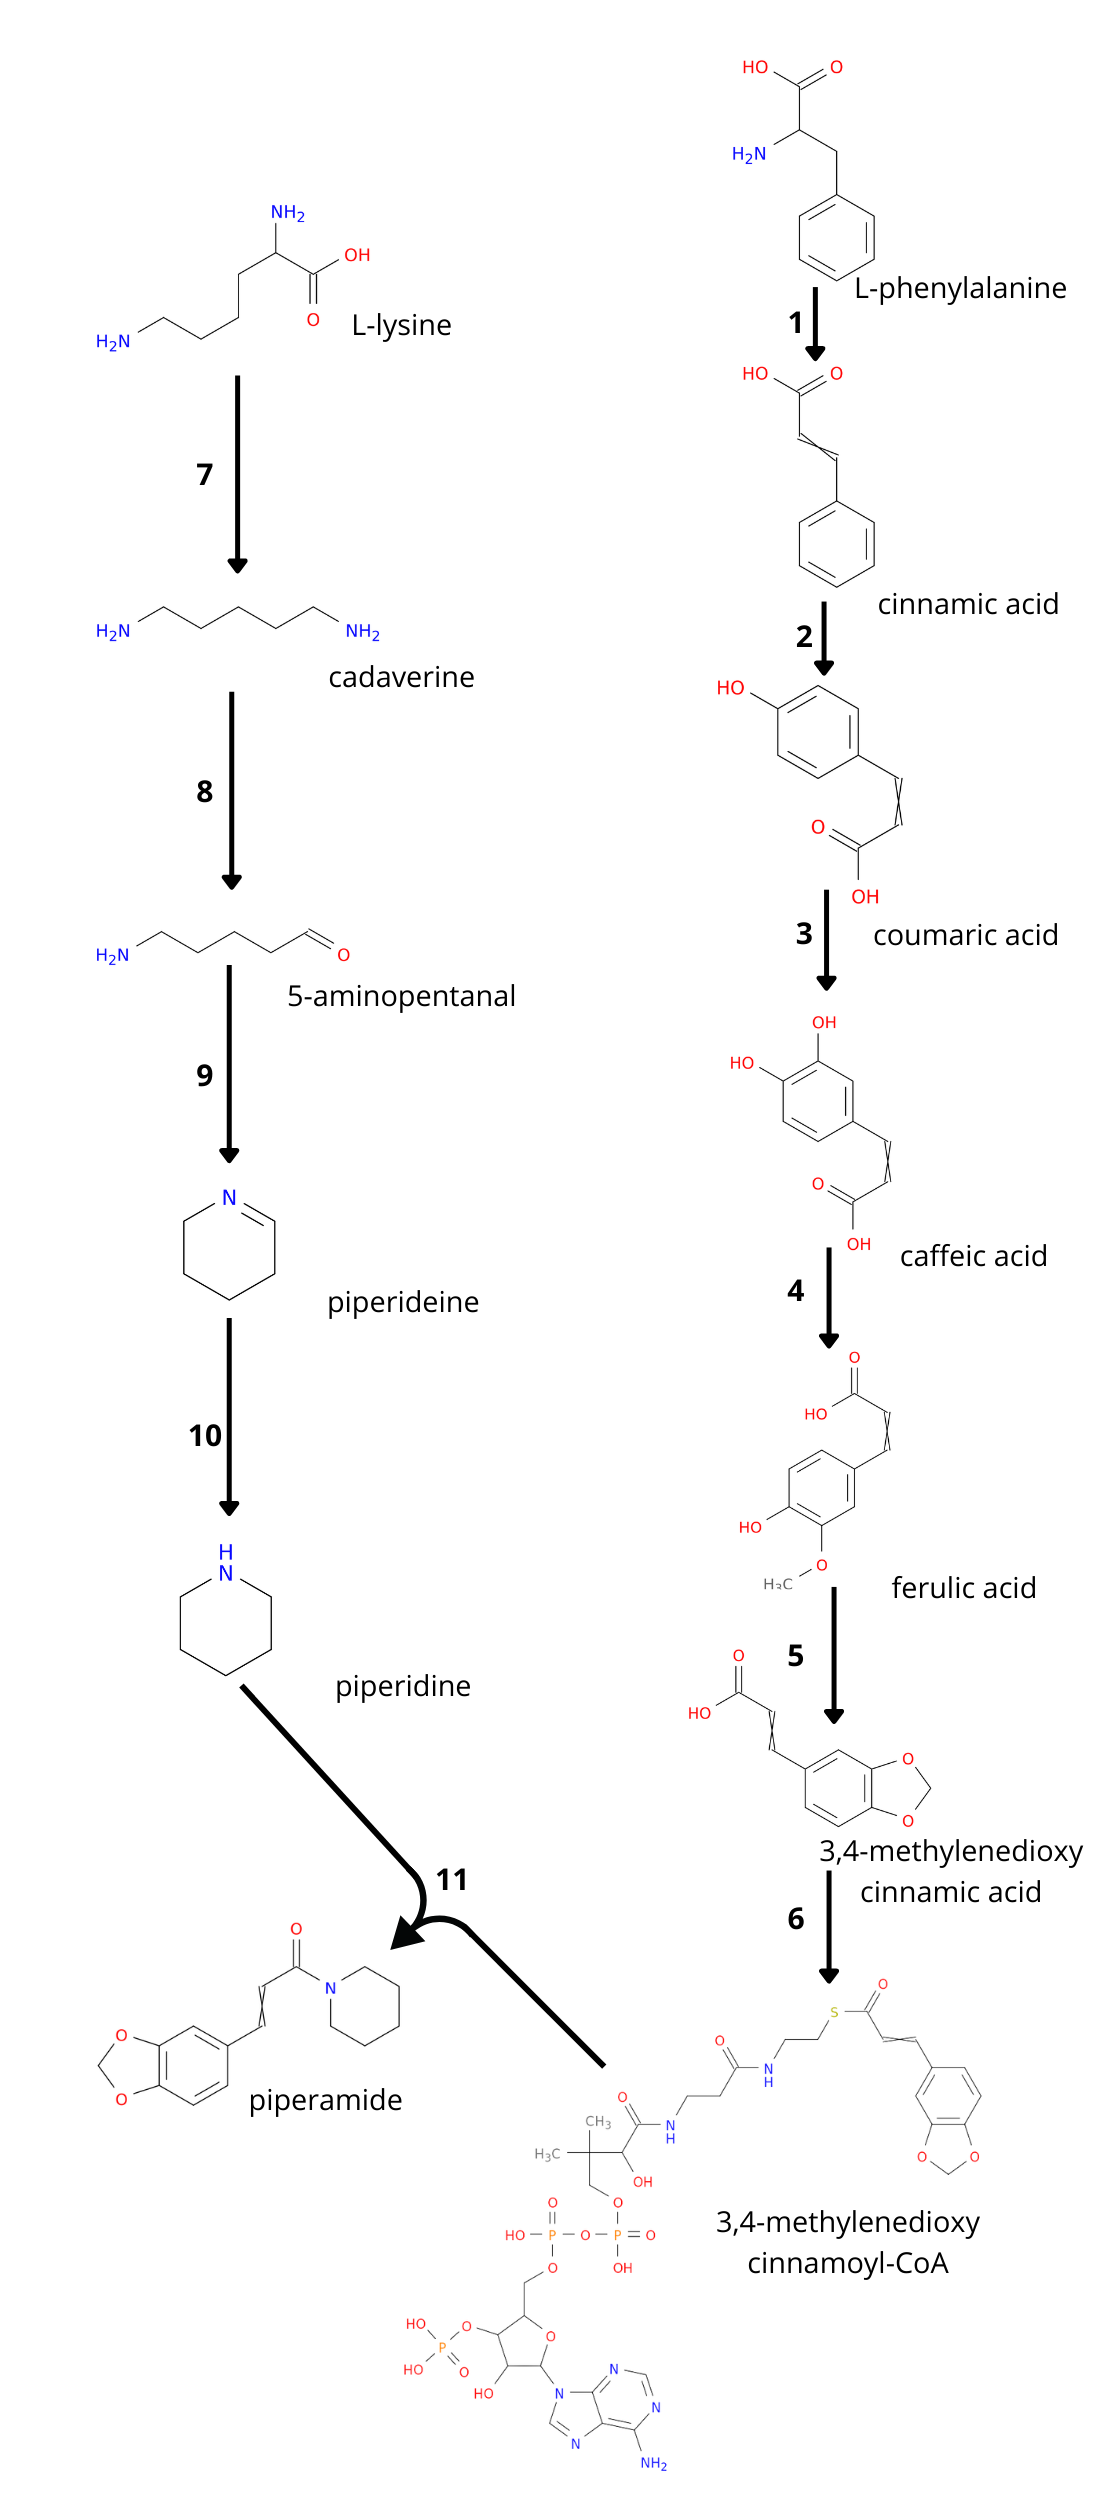
\includegraphics[scale=0.35]{Pathway2.png}
		\caption*{Biosynthetic pathway of piperamide.}
		
	\end{figure}
	\FloatBarrier
	
	
	\section{Docking}
	
	\subsection{Pn8.2617}
	
	The first reaction in the biosynthetic pathway of piperamide is performed by the enzyme phenylalanine ammonia-lyase, which is part of the phenylpropanoid biosynthesis pathway and catalyzes the reaction shown in Eq. \ref{eq1}. The gene Pn8.2617 was selected as the best candidate for enzyme 1, this selection was based on the fact that it obtained the highest score (1170.9) over the threshold (524.93) for KEGG Orthology ID K10775, with E-value $\approxeq 0$ . This annotation was made with KofamKOALA. \cite{kofamkoala} With the exon usage analysis no relevant results were found.
	
	
	\begin{equation}
		\schemestart
		 \label{eq1}
		\chemname{\footnotesize\chemfig{O=[:90](-[:30,,,1]OH)-[:150](-[:90,,,1]NH_2)-[:210]-[:150]-[:90]%
-[:150]-[:210](-[:330,,,,draw=none]\mcfcringle{1.3})-[:270]-[:330](-[:30])}
}{Phenylalanine}\arrow{->[ 1]}\chemname{\footnotesize\chemfig{O=[:90](-[:30,,,1]OH)-[:150]-[:210,,,,drh]-[:150]-[:90]-[:150]%
-[:210](-[:330,,,,draw=none]\mcfcringle{1.3})-[:270]-[:330](-[:30])}
}{Cinnamic acid}
		\arrow{0}[,0]+
		\chemname{\footnotesize\chemfig{NH_3}}{Ammonia}
		\schemestop
	\end{equation}\\
	
	\FloatBarrier
	\begin{wrapfigure}{r}{0.5\textwidth}
		\centering
		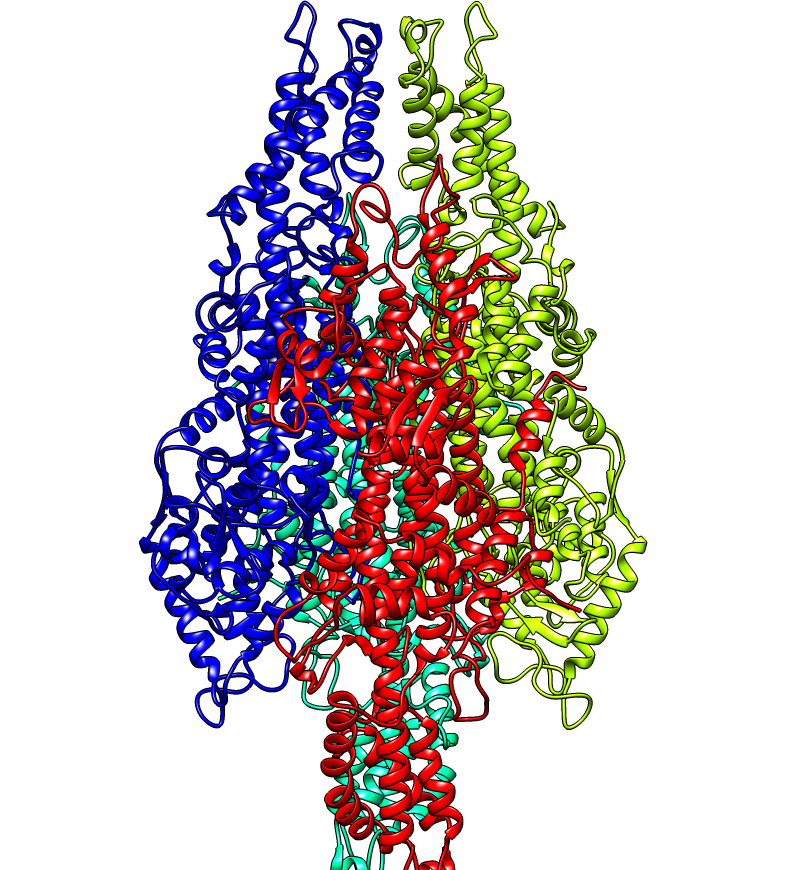
\includegraphics[width=0.5\textwidth]{../1/Minimize/model.png}
		\caption{Pn8.2617 three-dimensional model.}
		\label{fig1_1}
	\end{wrapfigure}
	\FloatBarrier
	
	The gene contains two exons that were considered when modeling the three-dimensional structure of the protein. The structure modeling was made by using an homology based methodology ``SWISS-MODEL''. \cite{swiss,quaternary_swiss} This methodology is template based, in this case the template selected was a phenylalanine ammonia-lyase from \textit{Petroselinum crispum} with PDB ID: \href{https://www.rcsb.org/structure/1w27}{1w27}; this protein has a 79.97\% sequence identity to our query protein Pn8.2617 which makes it an appropriate template. The template was found with HHblits, a protein sequence searching algorithm that uses hmm-hmm alignment. \cite{hhblits} The model (Fig. \ref{fig1_1}) is found in a homo-tetrameric state, as the template is; it has a GMQE value of 0.84 and a QMEANDisCo Global value of 0.81 ± 0.05 (Fig. \ref{fig1_2}). The QMEANDisCo value is a composite score value for single model quality estimation, this value is a function of underlying single model scores employing statistical potentials of mean force and a distance constraint based on the known structure of homologous proteins. QMEANDisCo value is calculated for every residue of the protein and the QMEANDisCo Global value is the average of these per residue scores, which aims to be a good approximation of the global overall quality of the model. \cite{qmeandisco_swiss} The ligand 3D conformer structure was obtained from PubChem with CID: \href{https://pubchem.ncbi.nlm.nih.gov/compound/6140}{6140}.

	
	\FloatBarrier
	\begin{figure}[h!]
		\centering
		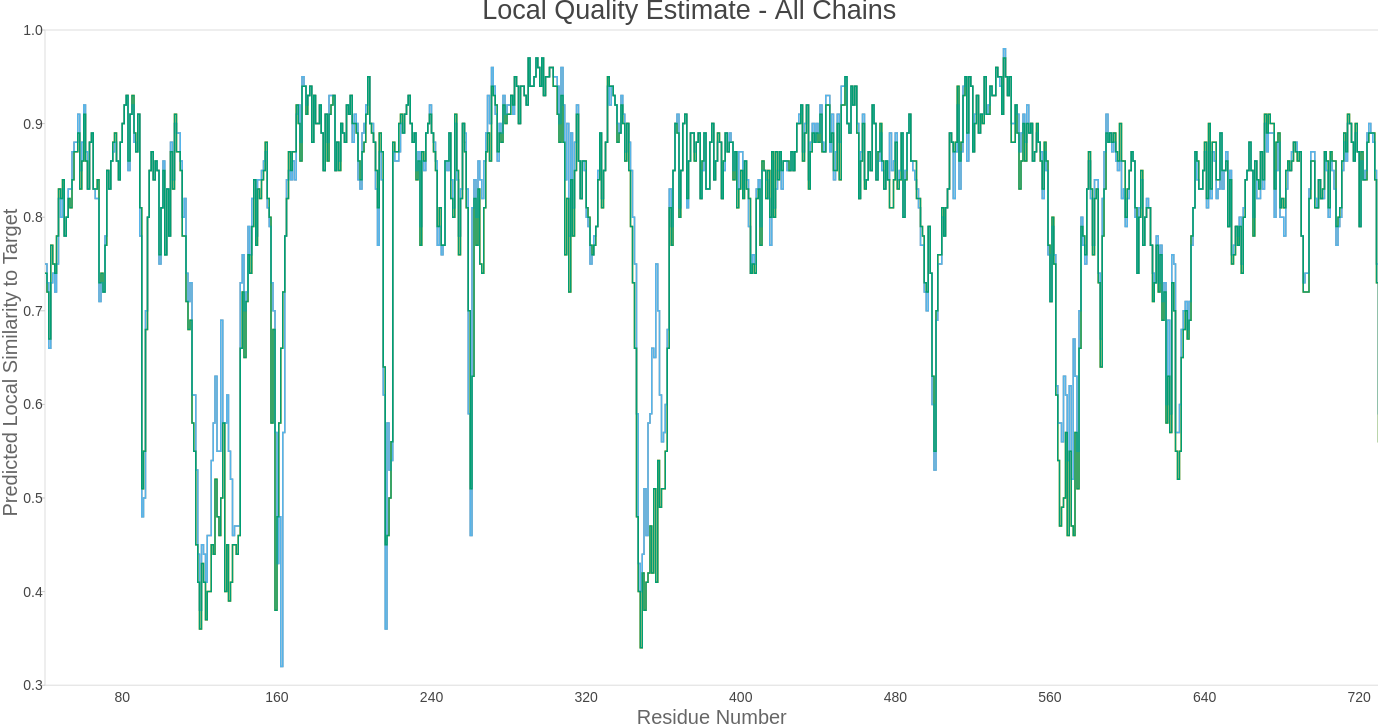
\includegraphics[width=\textwidth-50pt]{../1/Swiss/Local_quality_estimate.png}
		\caption{Pn8.2617 model QMEANDisCo.}
		\label{fig1_2}
	\end{figure}
	\FloatBarrier
	
	Before docking was performed the protein and the ligand were energy minimized. The protein structure was minimized using UCSF ChimeraX software \cite{chimera,chimera_2} and the steepest descent algorithm for 1000 steps with a step size of 0.02 \r{A}; the force field AMBER ff14SB was used for standar residues, for non standard residues the semi-empirical AM1-BCC model that uses an additive bond charge corrections was selected since it has shown higher success rate than other force fields in docking methods. \cite{am1_bcc,am1_bcc_2,am1_bcc_3} In the same way the ligand was energy minimized by using using the python library ``rdkit'' and the MMFF94 force field implemented within it. \cite{rdkit,rdkit_mmff}
	
	The preparation of the molecules for docking was made on AutoDockTools and Autodock Vina version 1.2.3 docked the protein and the ligand. \cite{adt,vina,vina_2} The grid box for the docking was selected based on the conserved domains found with the NCBI conserved domain search interface; we found the tetramer interface and active site conserved domains for phenylalanine ammonia-lyase from the CDD database. \cite{cdd,cdd_2}.  CASTp3 found the protein's pockets, which are cavities on its surface into which solvent can enter; CASTp3 uses computational geometry to find these pockets mainly using Delaunay triangulation, alpha shape, and discrete flow. \cite{castp} As a result of molecular docking with Vina, nine different conformations of the ligand in the protein were found, these results are shown in Table \ref{table1}.
	
	The docked positions of the phenylalanine in the Pn8.2617 structure interacted with different aminoacid residues of the protein (Fig. \ref{fig1_3}). Some of these aminoacids were found in the conserved domain for the active site of the enzyme, like Phe 129, Leu 147, Leu 270, Asn 274, Tyr 365, Arg 368 and Asn 398; the rest of the aminoacids were not marked as conserved in the active site domain but were present in the pockets found by CASTp3: Phe 150, Leu 221, Phe 414, Lys 470, Glu 498, Asn 501 and Gln 502.
	
	\begin{table}[h!]
		\centering
		\caption{Docking results of phenylalanine in Pn8.2617}
		\label{table1}
		\begin{tabular}{cccc}
			\toprule
			\multirow{2}{*}{Mode} & Affinity & \multicolumn{2}{c}{Dist. from best mode}\\
			&  (kcal/mol) & RMSD l.b & RMSD u.b\\
			\midrule
			1 & -6.278   &     0.0   &     0.0\\
			2 & -6.126   &   2.278   &   2.795\\
			3 & -6.098   &   1.934   &   2.262\\
			4 & -6.095   &   1.773   &   1.908\\
			5 & -6.013   &   1.735   &   2.332\\
			6 & -5.850   &   2.656   &   3.643\\
			7 & -5.847   &   1.749   &   2.333\\
			8 & -5.700   &   2.823   &   3.134\\
			9 & -5.670   &   3.526   &   4.412\\
			\bottomrule
			
		\end{tabular}
	\end{table}

	A further analysis was carried out to elucidate the protein-ligand interactions of the best conformation obtained, which has a binding energy of -6.278 kcal/mol. A search for hydrogen bonds was performed using UCSF ChimeraX allowing relax constraints of 0.4 \r{A} and 20 degrees, the bonds are shown as pseudobonds since they represent significant interactions between atoms other than covalent bonds, also because of the relax constraint these predictions can represent bonds within the tolerance values but not meeting the precise criteria. \cite{chimera,chimera_2,hbond} Four pseudobonds were found between the ligand and two aminoacids of the protein, one pseudobond with Asn 501 and a distance of 2.022 \r{A} and three with Arg 368 with distances of 2.240 \r{A}, 2.322 \r{A} and 2.438 \r{A}. In Fig. \ref{fig1_4} this pseudobonds and the ligand in its pocket are shown, the surface of the protein is colored based on its hydrophobicity using Kyte-Doolittle scale from lower (blue) to higher hydrophobicity (red).


	\FloatBarrier
	\begin{figure}[h!]
		\centering
		\begin{subfigure}[h!]{0.35\textwidth}
			\hspace{2cm}
			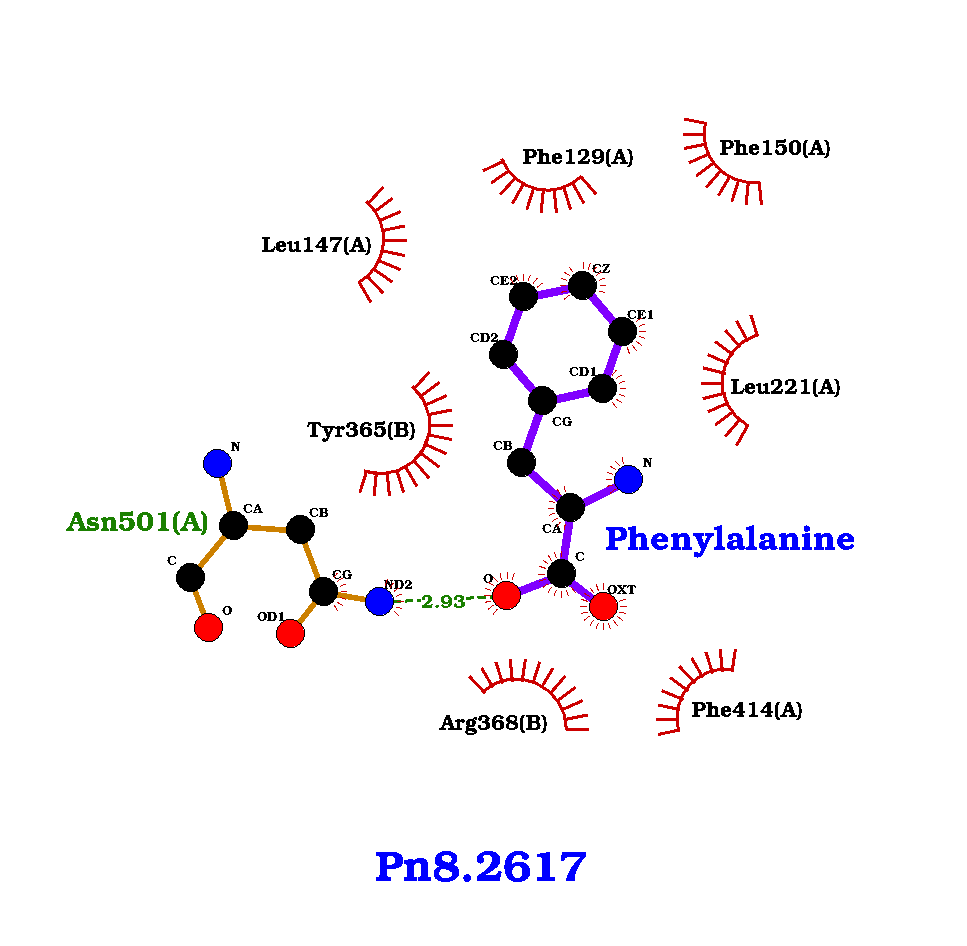
\includegraphics[width=\textwidth]{../1/Dock/best.png}
			\caption{}
		\end{subfigure}
		\hfill
		\begin{subfigure}[h!]{0.35\textwidth}
			\hspace{-2cm}
			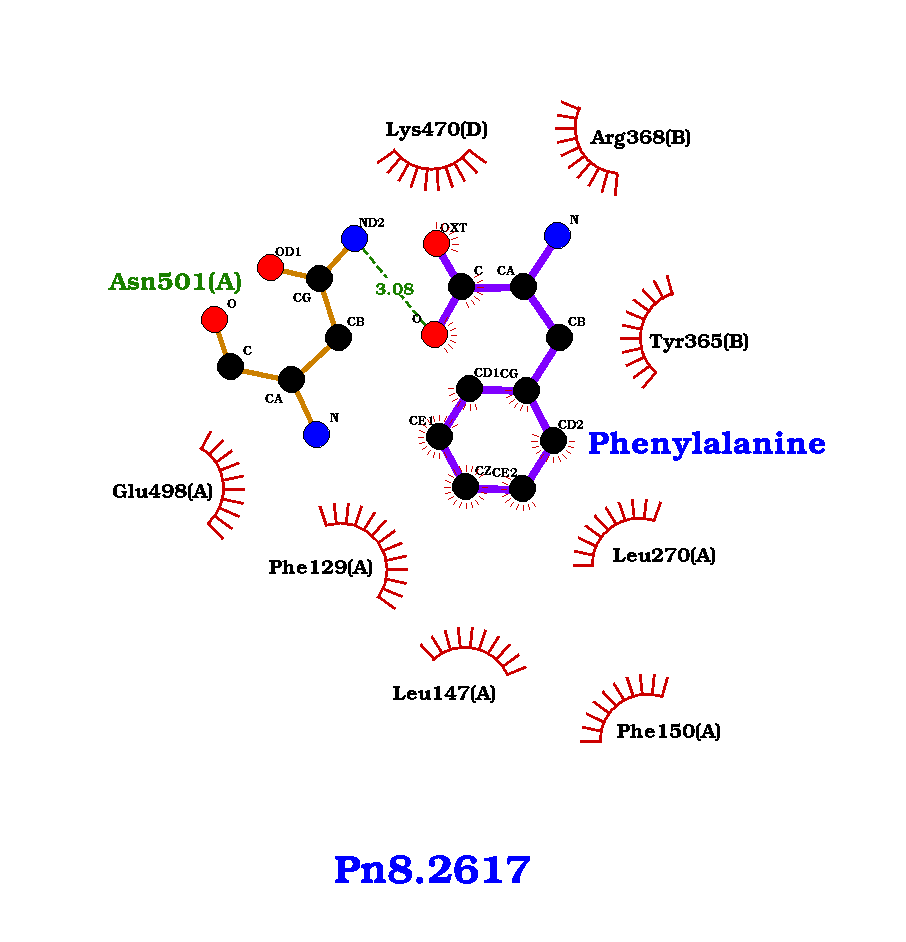
\includegraphics[width=\textwidth]{../1/Dock/best2.png}
			\caption{}
		\end{subfigure}
		\hfill
		\begin{subfigure}[h!]{0.35\textwidth}
			\hspace{2cm}
			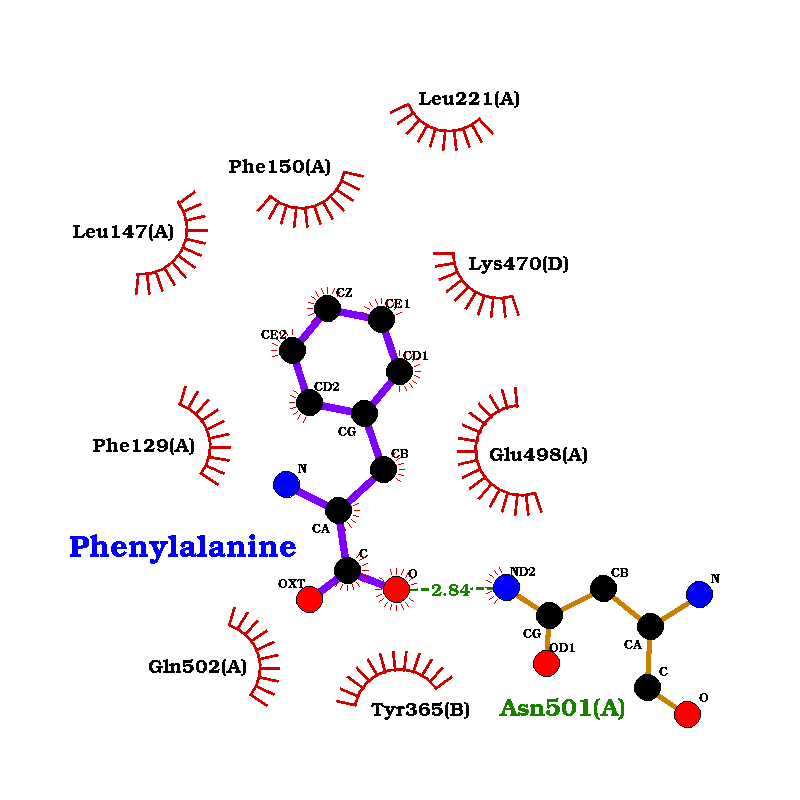
\includegraphics[width=\textwidth]{../1/Dock/best3.png}
			\caption{}
		\end{subfigure}
		\hfill
		\begin{subfigure}[h!]{0.35\textwidth}
			\hspace{-2cm}
			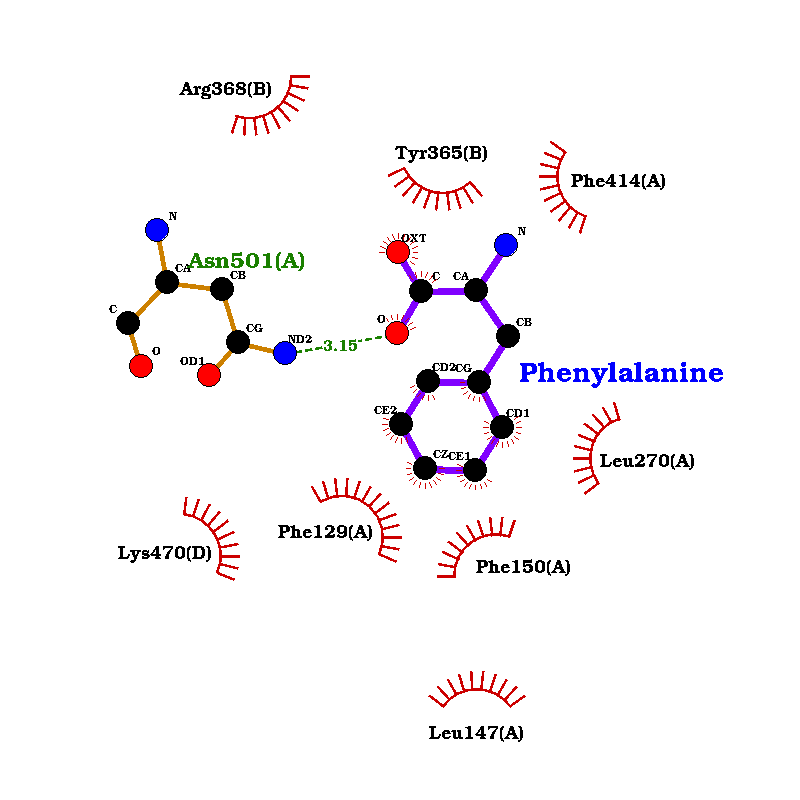
\includegraphics[width=\textwidth]{../1/Dock/best4.png}
			\caption{}
		\end{subfigure}
		\hfill
		\caption[Interactions between phenylalanine and Pn8.2617]{Interactions of phenylalanine with Pn8.2617. Best four poses are shown in order a-d.}
		\label{fig1_3}
	\end{figure}
	\FloatBarrier
	
	\FloatBarrier
	\begin{figure}[h!]
		\centering
		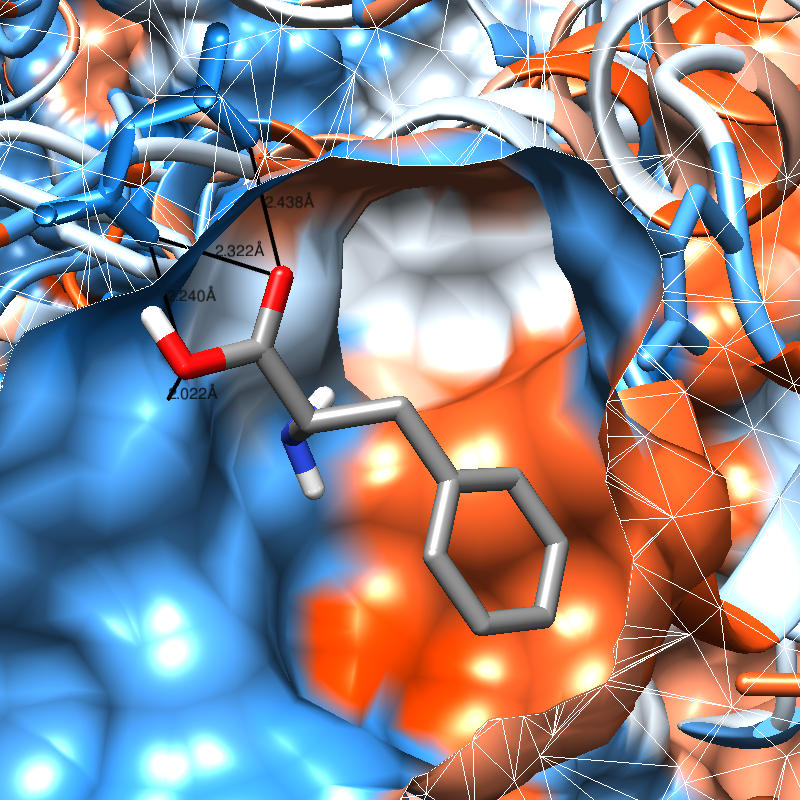
\includegraphics[width=0.4\textwidth]{../1/Dock/chimera.png}
		\caption{Phenylalanine pseudobonds with Pn8.2617.}
		\label{fig1_4}
	\end{figure}
	\FloatBarrier
	
	\subsection{Pn2.84}\label{ssec:Pn2.84}
	
	The second reaction of the pathway (Eq. \ref{eq2}) is catalyzed by a protein from the Cytochrome P450 Monooxigenase family called trans-cinnamate 4-hydroxylase, this enzyme is also part of the phenylpropanoid biosynthesis pathway. The gene Pn2.84 was selected as the best candidate for enzyme 2 based on the fact that it obtained the highest score (985.2) over the threshold (555.2) for KEGG Orthology ID K00487, with E-value $=2.5\times10^{-297}$. This annotation was made with KofamKOALA. \cite{kofamkoala} With the exon usage analysis no relevant results were found.
	
	\begin{equation}
	\schemestart
	\label{eq2}
	\chemname{\footnotesize\chemfig{O=[:90](-[:30,,,1]OH)-[:150]-[:210,,,,drh]-[:150]-[:90]-[:150]%
-[:210](-[:330,,,,draw=none]\mcfcringle{1.3})-[:270]-[:330](-[:30])}
}{Cinnamic acid}\arrow{->[ 2]}\chemname{\footnotesize\chemfig{O=[:60](-[:120,,,2]HO)--[:300,,,,drh]--[:300]--[:60](-[,,,1]OH)%
-[:120]-[:180](-[:240])(-[:300,,,,draw=none]\mcfcringle{1.3})}
}{Coumaric acid}
	\schemestop
	\end{equation}\\
	
	\FloatBarrier
	\begin{wrapfigure}{r}{0.5\textwidth}
		\centering
		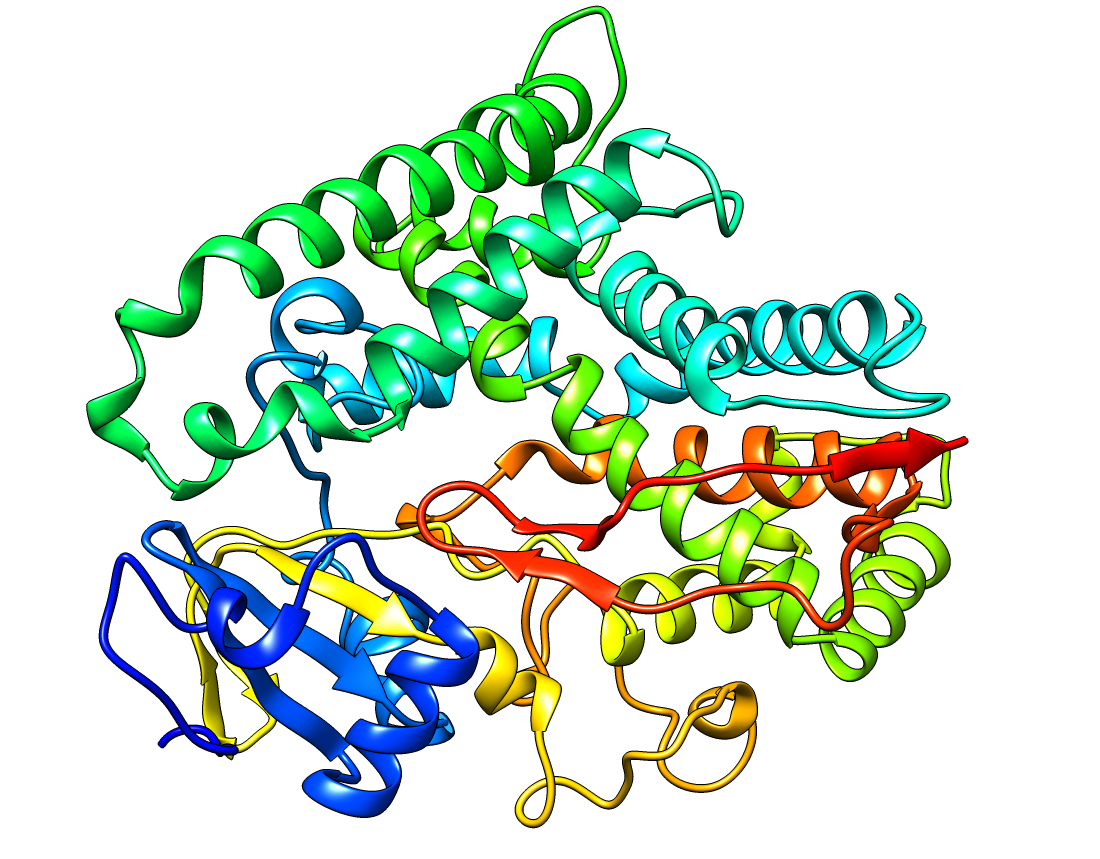
\includegraphics[width=0.5\textwidth]{../2/Minimize/model.png}
		\caption{Pn2.84 three-dimensional model.}
		\label{fig2_1}
	\end{wrapfigure}
	\FloatBarrier
	
	The gene contains four exons that were considered when modeling the three-dimensional structure of the protein. The structure modeling was made by using an homology based methodology ``SWISS-MODEL''. \cite{swiss} The selected template was a cinnamate 4-hydroxylase from \textit{Sorghum bicolor} with PDB ID: \href{https://www.rcsb.org/structure/6VBY}{6VBY}; this protein has a 77.91\% sequence identity to our query protein Pn2.84 which makes it an appropriate template. The template was found with HHblits, a protein sequence searching algorithm that uses hmm-hmm alignment. \cite{hhblits} The model (Fig. \ref{fig2_1}) is found in a monomeric state, as the template is; it has a GMQE value of 0.91 and a QMEANDisCo Global value of 0.91 ± 0.05 (Fig. \ref{fig2_2}). \cite{qmeandisco_swiss} The enzyme requires an heme molecule as a coenzyme for its correct catalytic activity; in the template a protoporphyrin IX containing Fe was found, which was used as a coenzyme for Pn2.84. The ligand 3D conformer structure was obtained from PubChem with CID: \href{https://pubchem.ncbi.nlm.nih.gov/compound/5957728}{5957728}.
	
	
	\FloatBarrier
	\begin{figure}[h!]
		\centering
		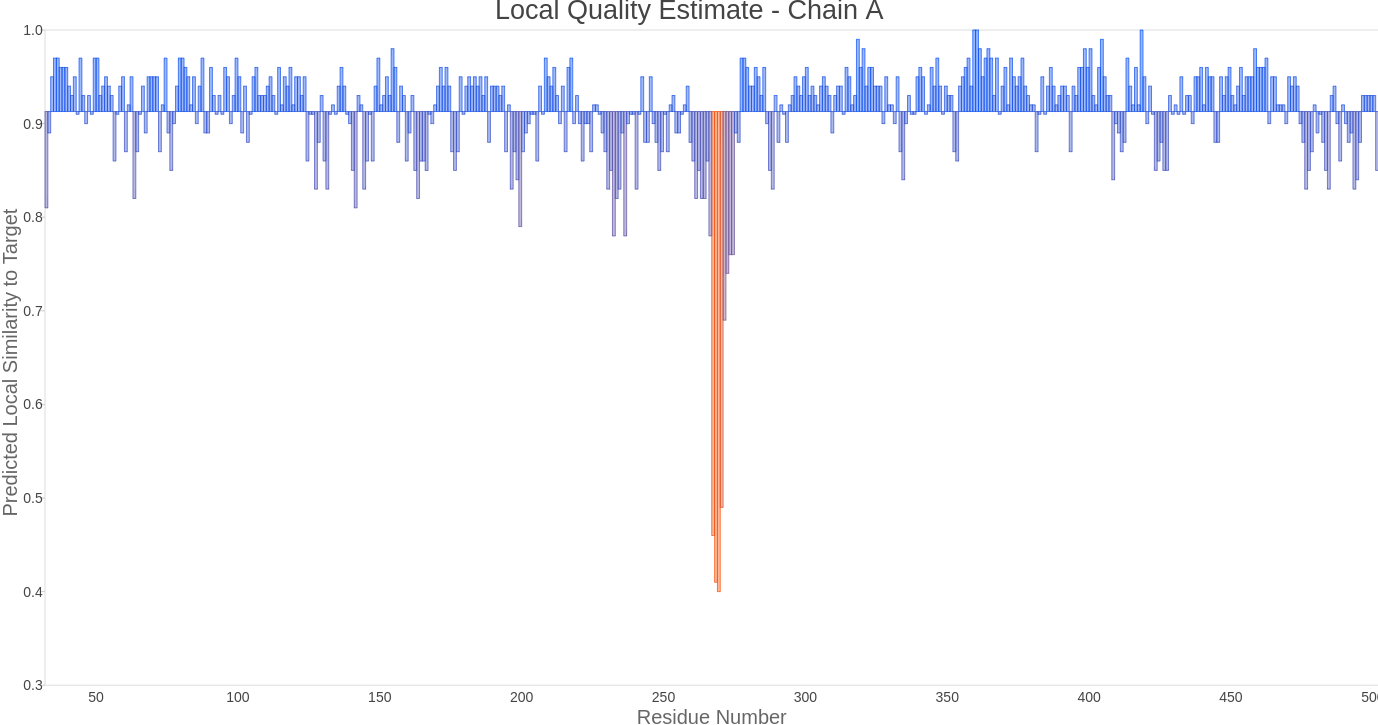
\includegraphics[width=\textwidth-50pt]{../2/Swiss/Local_quality_estimate.png}
		\caption{Pn2.84 model QMEANDisCo.}
		\label{fig2_2}
	\end{figure}
	\FloatBarrier
	
	Before docking was performed the protein and the ligand were energy minimized. The protein structure was minimized using UCSF ChimeraX software \cite{chimera,chimera_2} and the steepest descent algorithm for 1000 steps with a step size of 0.02 \r{A}; the force field AMBER ff14SB was used for standar residues, for non standard residues the semi-empirical AM1-BCC model. \cite{am1_bcc,am1_bcc_2,am1_bcc_3}\ \ In the same way the ligand was energy minimized by using using the python library ``rdkit'' and the MMFF94 force field implemented within it. \cite{rdkit,rdkit_mmff}
	
	The preparation of the molecules for docking was made on AutoDockTools and Autodock Vina version 1.2.3 docked the protein and the ligand. \cite{adt,vina,vina_2} The grid box for the docking was selected based on the conserved domains found with the NCBI conserved domain search interface; we found the heme binding site and putative chemical substrate binding pocket conserved domains for trans-cinnamate 4-hydroxylase from the NCBI-Curated Domains database; additionally, active site residues were selected from the template structure, which included mainly Arg 213, Ser 214 and Gln 218. \cite{cdd,cdd_2}.  CASTp3 found the protein's pockets. \cite{castp} To perform an adequate docking of both the heme group and the cinnamate molecule a sequential docking workflow was used as described in \textcite{sequential}; in this methodology the protein and ligand were prepared (energy minimized) before the docking was performed, then the first molecule was  docked to the protein, the best pose was merged with the protein and this complex was used as a the receptor to dock the next compound.
	
	\newpage
	\subsubsection{Protoporphyrin IX with Fe}
	
	The first molecule docked was the protoporphyrin IX with Fe, as a result of molecular docking with Vina, nine different conformations of the molecule in the protein were found, these results are shown in Table \ref{table2_1}. The docked positions of the protoporphyrin IX with Fe in the Pn2.84 structure interacted with different aminoacid residues of the protein (Fig. \ref{fig2_3}). Some of these aminoacids were found in the conserved domain for the heme binding site of the enzyme, like Arg 101, Trp 126, Arg 130, Phe 138, Met 186, Ile 303, Ala 306, Ala 307, Thr 310, Thr 311, Leu 374, Val 375, His 377, Pro 439, Phe 440, Gly 441, Arg 445, Ser 446, Cys 447, Pro 448, Gly 449, Leu 452, and Ala 453; the rest of the aminoacids were not marked as conserved in the heme binding site domain but were present in the pockets found by CASTp3: Leu 91, Met 117, Val 118, Met 133, Ser 314, Ile 365, Ile 371 and Leu 457.
	
	
	\begin{table}[h!]
		\centering
		\caption{Docking results of protoporphyrin IX (Fe) with Pn2.86}
		\label{table2_1}
		\begin{tabular}{cccc}
			\toprule
			\multirow{2}{*}{Mode} & Affinity & \multicolumn{2}{c}{Dist. from best mode}\\
			&  (kcal/mol) & RMSD l.b & RMSD u.b\\
			\midrule
			1 & -9.795   &       0   &       0.0\\
			2 &  -8.72   &  0.7843   &     6.157\\
			3 & -8.471   &   2.831   &     7.051\\
			4 & -8.274   &   3.895   &     8.459\\
			5 & -7.935   &   2.005   &     4.936\\
			6 & -7.545   &   2.033   &      6.57\\
			7 &  -6.66   &   3.496   &     8.093\\
			8 & -6.646   &   3.464   &     7.518\\
			9 & -6.506   &   2.739   &     6.189\\
			\bottomrule
			
		\end{tabular}
	\end{table}

	A further analysis was carried out to elucidate the protein-ligand interactions of the best conformation obtained, which has a binding energy of -9.795 kcal/mol. A search for hydrogen bonds was performed using UCSF ChimeraX allowing relax constraints of 0.4 \r{A} and 20 degrees. \cite{chimera,chimera_2,hbond} Eight pseudobonds were found between the ligand and four aminoacids of the protein: three pseudobonds with Arg 101 with distances 2.033 \r{A}, 2.169 \r{A} and 2.206 \r{A}; one pesudobond with Trp 126 of 2.197 \r{A}; one with His 377 of 2.104 \r{A}; and three with Arg 445 with distances 1.964 \r{A}, 2.128 \r{A} and 2.238 \r{A}. In Fig. \ref{fig2_4} this pseudobonds and the ligand in its pocket are shown, the surface of the protein is colored based on its hydrophobicity using Kyte-Doolittle scale from lower (blue) to higher hydrophobicity (red).

	\FloatBarrier
	\begin{figure}[h!]
		\centering
		\begin{subfigure}[h!]{0.35\textwidth}
			\hspace{2cm}
			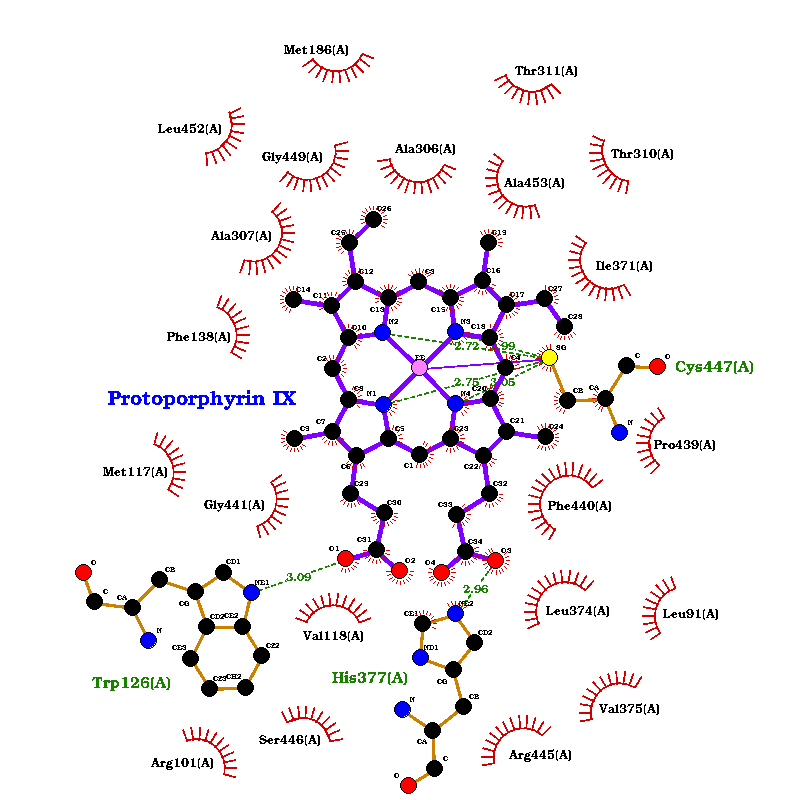
\includegraphics[width=\textwidth]{../2/Dock/best.png}
			\caption{}
		\end{subfigure}
		\hfill
		\begin{subfigure}[h!]{0.35\textwidth}
			\hspace{-2cm}
			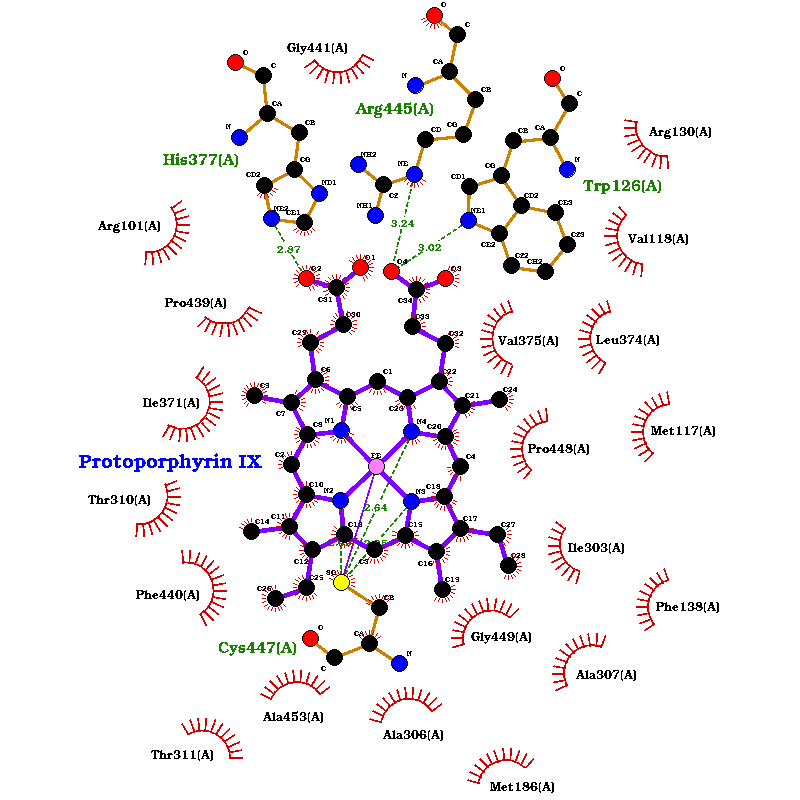
\includegraphics[width=\textwidth]{../2/Dock/best2.png}
			\caption{}
		\end{subfigure}
		\hfill
		\begin{subfigure}[h!]{0.35\textwidth}
			\hspace{2cm}
			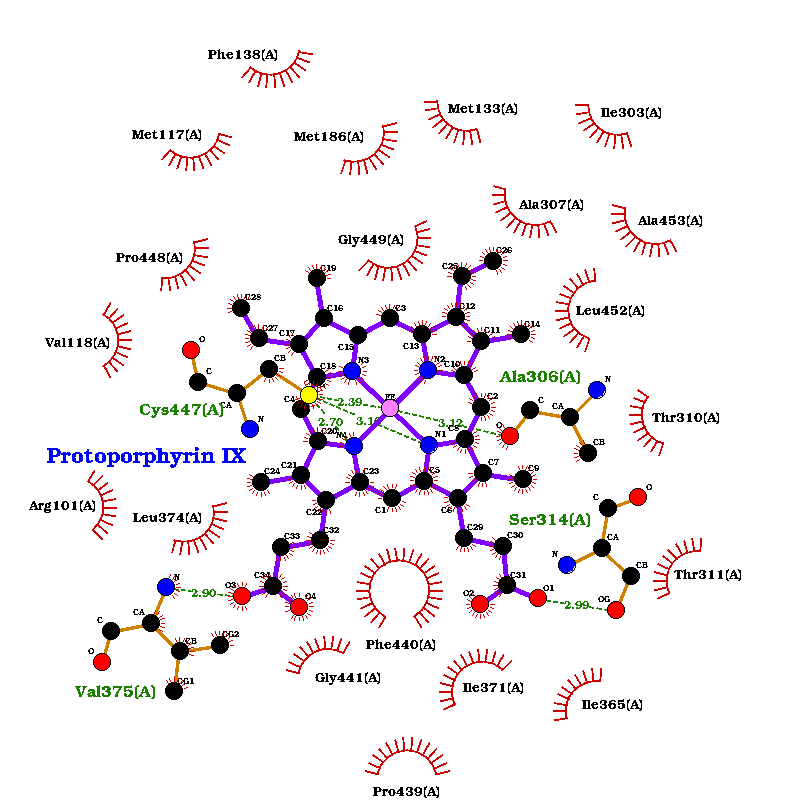
\includegraphics[width=\textwidth]{../2/Dock/best3.png}
			\caption{}
		\end{subfigure}
		\hfill
		\begin{subfigure}[h!]{0.35\textwidth}
			\hspace{-2cm}
			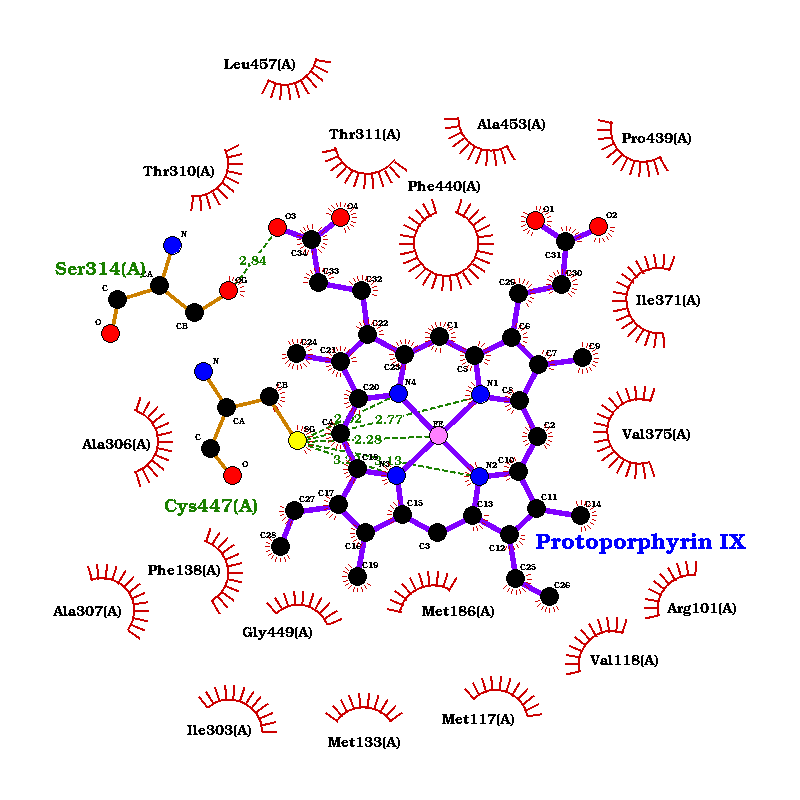
\includegraphics[width=\textwidth]{../2/Dock/best4.png}
			\caption{}
		\end{subfigure}
		\hfill
		\caption[Interactions between protoporphyrin IX with Fe and Pn2.84]{Interactions of protoporphyrin IX with Fe and Pn2.84. Best four poses are shown in order a-d.}
		\label{fig2_3}
	\end{figure}
	\FloatBarrier
	
	\FloatBarrier
	\begin{figure}[h!]
		\centering
		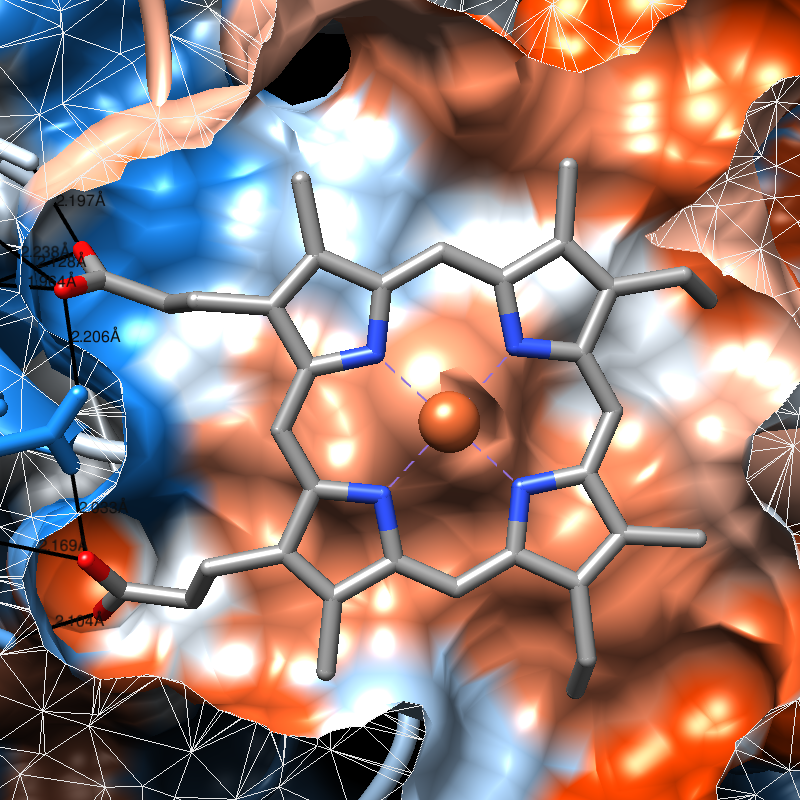
\includegraphics[width=0.4\textwidth]{../2/Dock/chimera.png}
		\caption{Protoporphyrin IX pseudobonds with Pn2.84.}
		\label{fig2_4}
	\end{figure}
	\FloatBarrier
	
	
	\subsubsection{Cinnamic acid}
	
	With the Pn2.84 protein and the best docked pose of protoporphyrin IX with Fe as a complex, molecular docking using Vina was carried out for trans-cinnamic acid resulting in nine different conformations, these results are shown in Table \ref{table2_2} The docked positions of the trans-cinnamic acid in the receptor structure interacted with different aminoacid residues of the protein (Fig. \ref{fig2_5}). Some of these aminoacids were found in the conserved domain for the active site of the enzyme, like Phe 107, Val 118, Phe 119, Arg 213, Ser 214, Gln 218, Val 305, Ala 306, Ile 371 and Val 375; the rest of the aminoacids were not marked as conserved in the active site domain but were present in the pockets found by CASTp3: Thr 310, Trp 313, Leu 374, Pro 376 and Phe 488.
	
	\begin{table}[h!]
		\centering
		\caption{Docking results of cinnamic acid with protoporphyrin IX-Pn2.86 complex}
		\label{table2_2}
		\begin{tabular}{cccc}
			\toprule
			\multirow{2}{*}{Mode} & Affinity & \multicolumn{2}{c}{Dist. from best mode}\\
			&  (kcal/mol) & RMSD l.b & RMSD u.b\\
			\midrule
			1 &  -6.66   &       0   &         0\\
			2 & -6.359   &   2.652   &     3.093\\
			3 & -6.147   &   1.105   &     1.982\\
			4 & -5.586   &   2.381   &     2.985\\
			5 & -5.577   &   3.276   &     5.403\\
			6 &  -5.57   &   3.049   &     3.496\\
			7 & -5.414   &   5.377   &     5.865\\
			8 & -5.291   &   2.987   &     3.666\\
			9 & -5.271   &   4.219   &     5.511\\
			\bottomrule
			
		\end{tabular}
	\end{table}

	A search for hydrogen bonds was performed with the best conformation (-6.66 kcal/mol) using UCSF ChimeraX allowing relax constraints of 0.4 \r{A} and 20 degrees. \cite{chimera,chimera_2,hbond} Four pseudobonds were found between the ligand and four aminoacids of the protein: two pseudobonds with Arg 213 with distances 2.378 \r{A} and 2.539 \r{A}; one pesudobond with Ser 214 of 2.329 \r{A}; and one with Gln 218 of 2.312 \r{A}. In Fig. \ref{fig2_6} this pseudobonds and the ligand in its pocket are shown, also the distance between the trans-cinnamate and the Fe atom of the heme group is represented; the surface of the protein is colored based on its hydrophobicity using Kyte-Doolittle scale from lower (blue) to higher hydrophobicity (red). Reliability of the docking is supported by the fact that strong interactions between cinnamic acid and aminoacid residues Arg 213, Ser 214 and Gln 218 were found, consistent with what is found in the template crystal structure and the conserved domain for the active site. The interaction found between the cinnamic acid and the heme group and the slightly smaller distance between the cinnamic acid and the Fe atom found in this analysis compared to \textcite{cinnamate_oxygenase} (4.142 \r{A} vs 4.4 \r{A}), provide also a strong support for this docking methodology.

	
	\FloatBarrier
	\begin{figure}[h!]
		\centering
		\begin{subfigure}[h!]{0.35\textwidth}
			\hspace{2cm}
			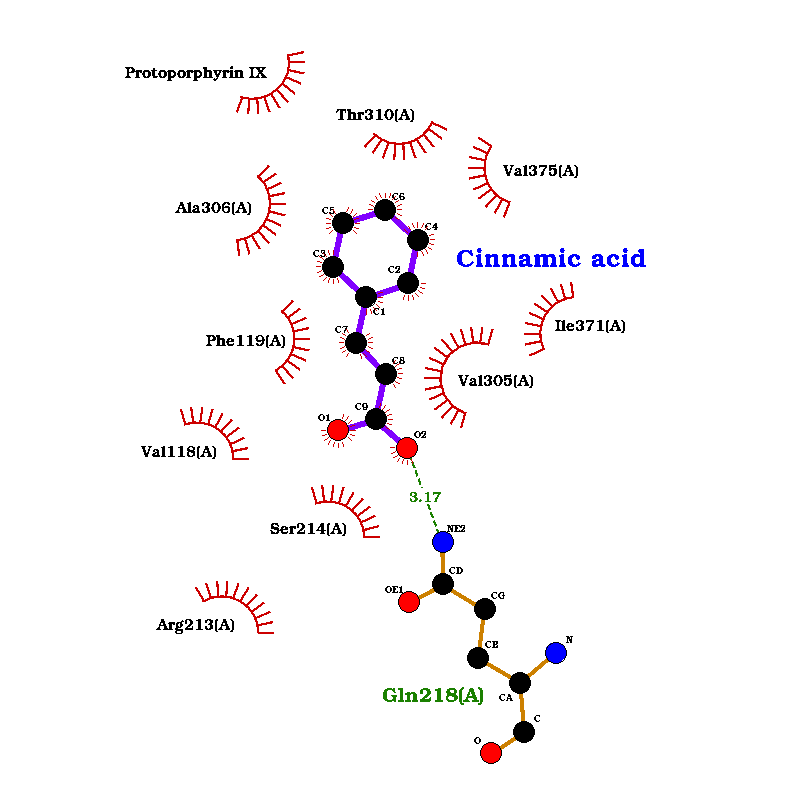
\includegraphics[width=\textwidth]{../2/Dock/Dock2/best.png}
			\caption{}
		\end{subfigure}
		\hfill
		\begin{subfigure}[h!]{0.35\textwidth}
			\hspace{-2cm}
			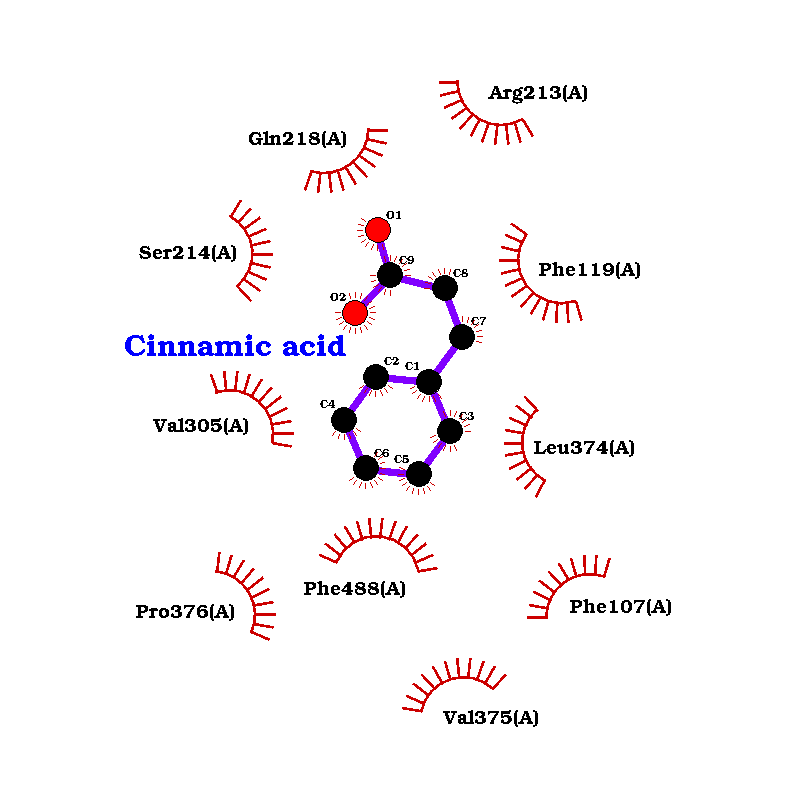
\includegraphics[width=\textwidth]{../2/Dock/Dock2/best2.png}
			\caption{}
		\end{subfigure}
		\hfill
		\begin{subfigure}[h!]{0.35\textwidth}
			\hspace{2cm}
			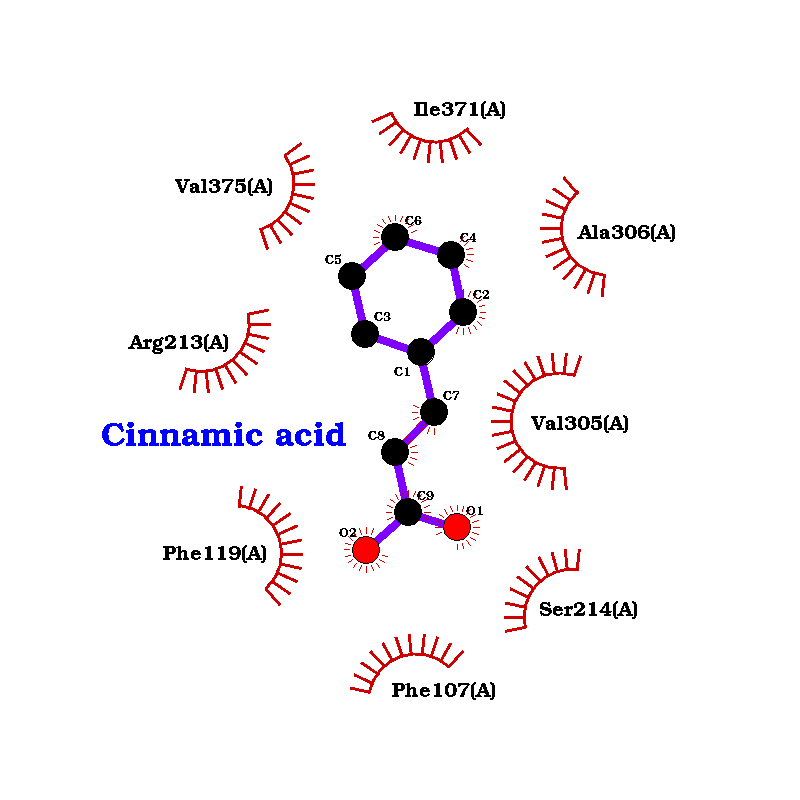
\includegraphics[width=\textwidth]{../2/Dock/Dock2/best3.png}
			\caption{}
		\end{subfigure}
		\hfill
		\begin{subfigure}[h!]{0.35\textwidth}
			\hspace{-2cm}
			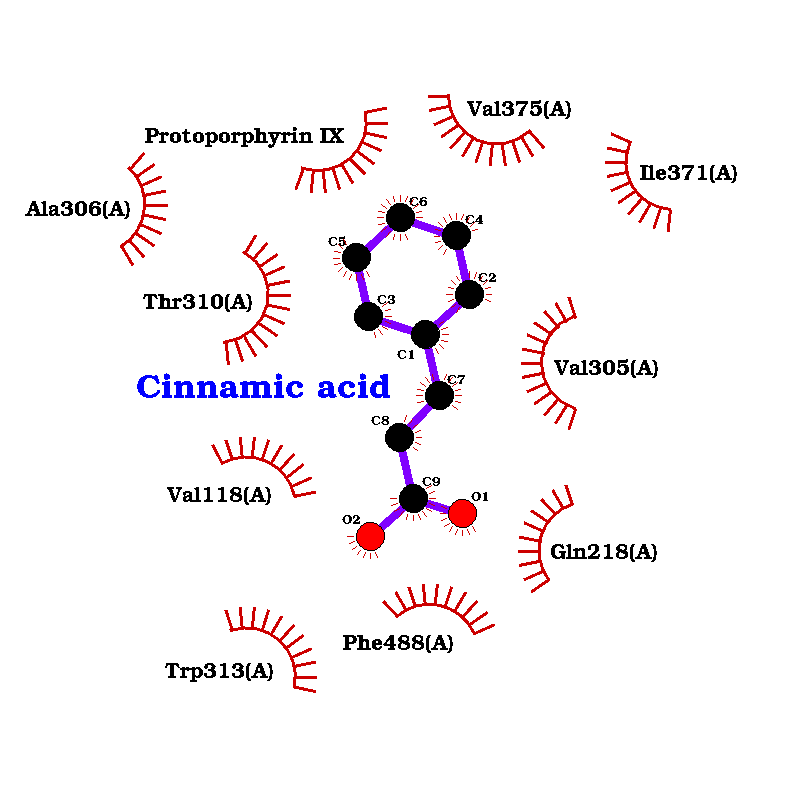
\includegraphics[width=\textwidth]{../2/Dock/Dock2/best4.png}
			\caption{}
		\end{subfigure}
		\hfill
		\caption[Interactions between cinnamic acid and protoporphyrin IX-Pn2.86 complex.]{Interactions of cinnamic acid with protoporphyrin IX-Pn2.86 complex. Best four poses are shown in order a-d.}
		\label{fig2_5}
	\end{figure}
	\FloatBarrier
	
	\FloatBarrier
	\begin{figure}[h!]
		\centering
		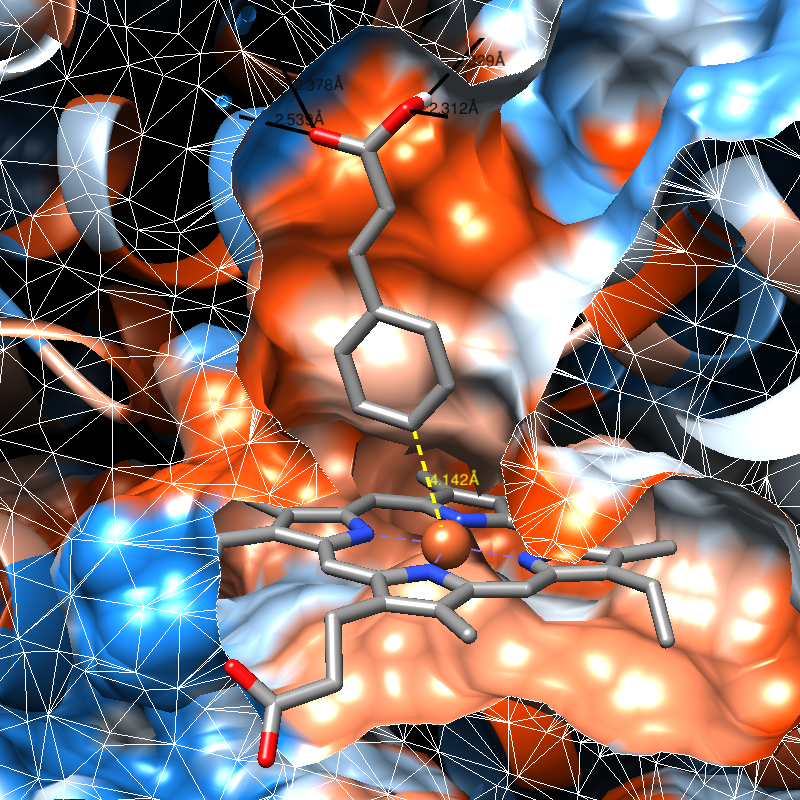
\includegraphics[width=0.4\textwidth]{../2/Dock/Dock2/chimera.png}
		\caption{Cinnamic acid pseudobonds with protoporphyrin IX-Pn2.86 complex.}
		\label{fig2_6}
	\end{figure}
	\FloatBarrier
	
	\subsection{Pn1.1317}
	
	The fourth reaction of the pathway (Eq. \ref{eq3}) is catalyzed by the protein caffeic acid 3-O-methyltransferase, this enzyme is also part of the phenylpropanoid biosynthesis pathway. The gene Pn1.1317 was selected as the best candidate for enzyme 4 based on the fact that it obtained the highest score (651.5) over the threshold (499.33) for KEGG Orthology ID K13066, with E-value $=2.9\times10^{-196}$. This annotation was made with KofamKOALA. \cite{kofamkoala} With the exon usage analysis no relevant results were found.
	
	\begin{equation}
	\schemestart
	\label{eq3}
	\chemname{\footnotesize\chemfig{O=[:90](-[:150,,,2]HO)-[:30]-[:330,,,,drh]-[:30]-[:330]-[:30](%
-[:330,,,1]OH)-[:90](-[:30,,,1]OH)-[:150]-[:210](-[:270])(%
-[:330,,,,draw=none]\mcfcringle{1.3})}
}{Caffeic acid}\arrow(caf--fer){-X>[][][4][SAM][SAH][]}\chemname{\footnotesize\chemfig{-[:270]O-[:210]-[:270](-[:330,,,1]OH)(%
-[:150,,,,draw=none]\mcfcringle{1.3})-[:210]-[:150]-[:90](-[:30]-[:330])%
-[:150]-[:210,,,,drh]-[:150](=[:90]O)-[:210,,,2]HO}
}{Ferulic acid}
	\schemestop
	\end{equation}\\
	
	
	\FloatBarrier
	\begin{wrapfigure}{r}{0.5\textwidth}
		\centering
		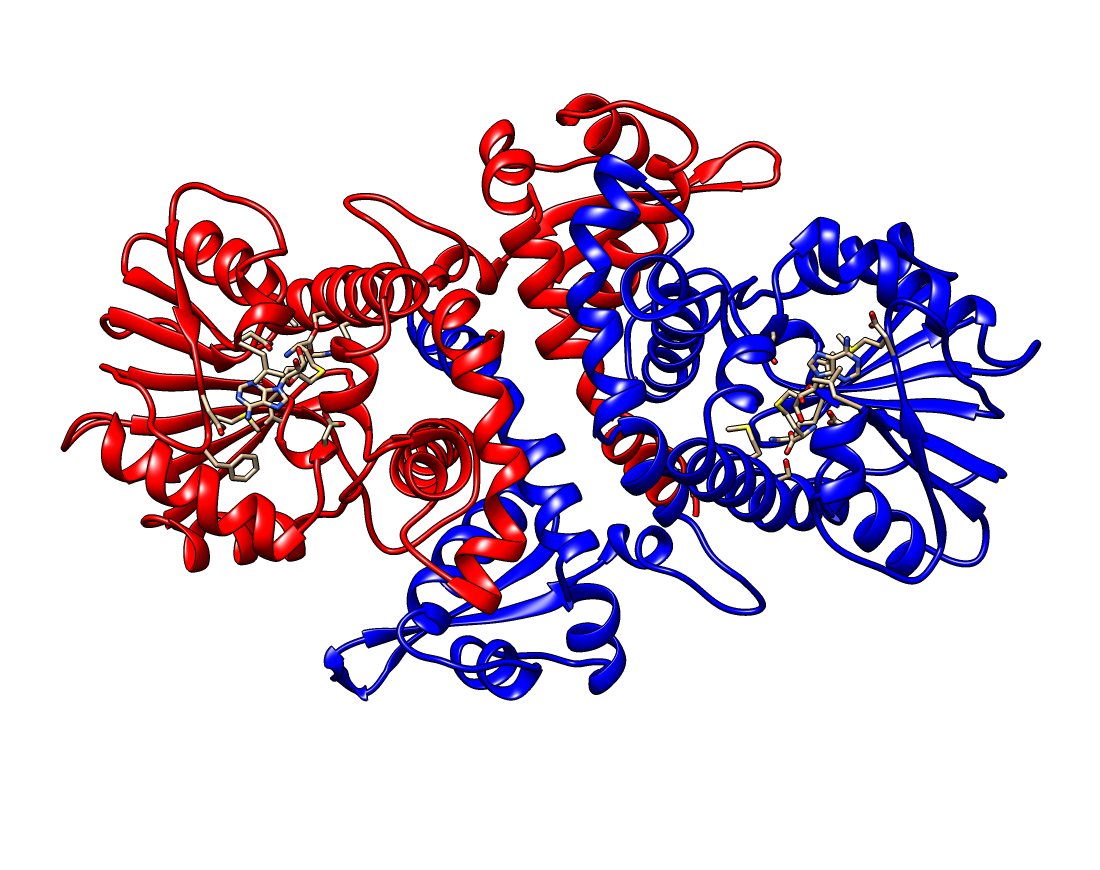
\includegraphics[width=0.5\textwidth]{../4/Swiss/model2.png}
		\caption{Pn2.84 three-dimensional model.}
		\label{fig4_1}
	\end{wrapfigure}
	\FloatBarrier
	
	The gene contains four exons that were considered when modeling the three-dimensional structure of the protein. The structure modeling was made by using an homology based methodology ``SWISS-MODEL''. \cite{swiss} The selected template was an O-methyltransferase from \textit{Fragaria ananassa} with PDB ID: \href{https://www.rcsb.org/structure/6I71}{6I71}; this protein has a 68.39\% sequence identity to our query protein Pn1.1317 which makes it an appropriate template. The template was found with HHblits. \cite{hhblits} The model (Fig. \ref{fig4_1}) is found in a dimeric state, as the template is; it has a GMQE value of 0.84 and a QMEANDisCo Global value of 0.81 ± 0.05 (Fig. \ref{fig4_2}). \cite{qmeandisco_swiss}	The enzyme requires a coenzyme SAM (S-adenosylmethionine) for its correct catalytic activity; this molecule is demethylated to SAH (S-adenosyl-L-homocysteine). The crystal structure of the template contained SAH binded to it, the biding site for SAH was conserved in Pn1.1317 so the model generated contained his molecule, the interactions between this ligand and the protein can be seen in Fig \ref{fig4_3}. The ligand 3D conformer structure for SAM and caffeic acid were obtained from PubChem with CIDs: \href{https://pubchem.ncbi.nlm.nih.gov/compound/34755}{34755} and \href{https://pubchem.ncbi.nlm.nih.gov/compound/689043}{689043}.
	
	\FloatBarrier
	\begin{figure}[h!]
		\centering
		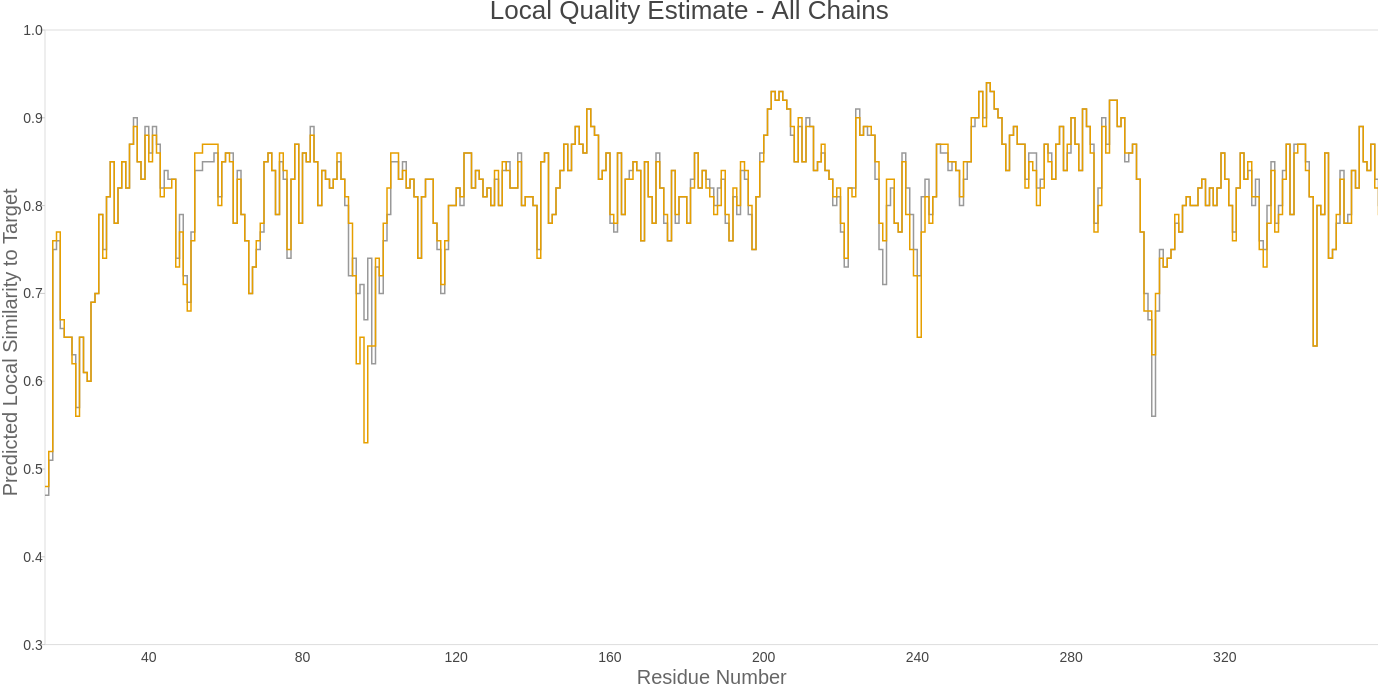
\includegraphics[width=\textwidth-50pt]{../4/Swiss/Local_quality_estimate.png}
		\caption{Pn1.1317 model QMEANDisCo.}
		\label{fig4_2}
	\end{figure}
	\FloatBarrier
	
	\FloatBarrier
	\begin{wrapfigure}{l}{0.5\textwidth}
		\centering
		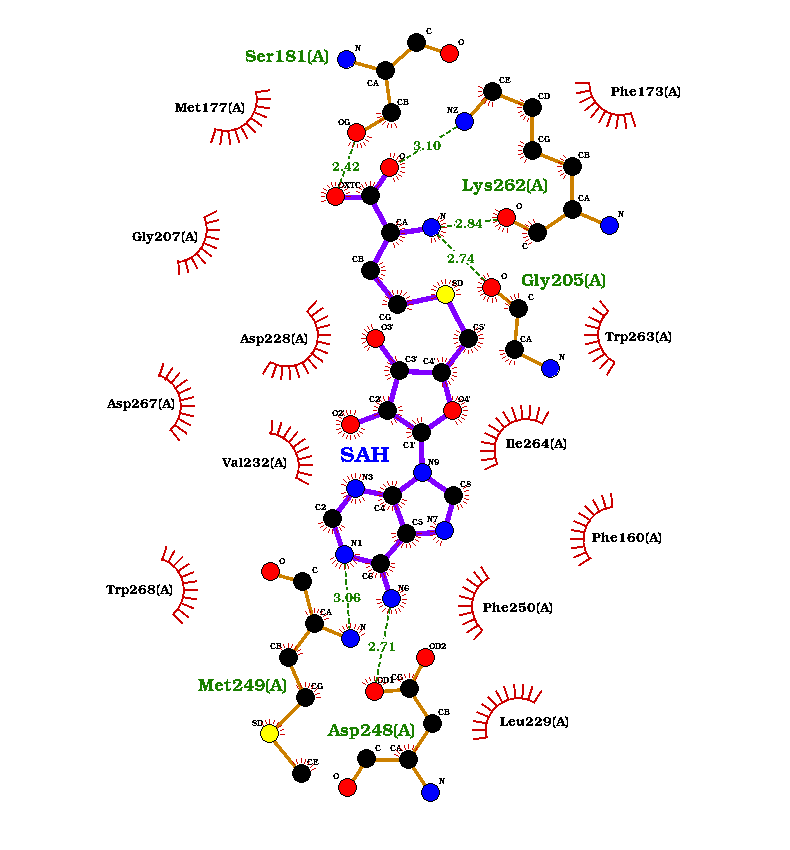
\includegraphics[width=0.5\textwidth]{../4/Swiss/sah.png}
		\caption{Interactions between SAH and Pn1.1317.}
		\label{fig4_3}
	\end{wrapfigure}
	\FloatBarrier
	
	Before docking was performed the protein and the ligand were energy minimized. The protein structure was minimized using UCSF ChimeraX software \cite{chimera,chimera_2} and the steepest descent algorithm for 1000 steps with a step size of 0.02 \r{A}; the force field AMBER ff14SB was used for standar residues, for non standard residues the semi-empirical AM1-BCC model. \cite{am1_bcc,am1_bcc_2,am1_bcc_3} In the same way the ligands were energy minimized by using using the python library ``rdkit'' and the MMFF94 force field implemented within it. \cite{rdkit,rdkit_mmff}
	
	The preparation of the molecules for docking was made on AutoDockTools and Autodock Vina version 1.2.3 docked the protein and the ligand. \cite{adt,vina,vina_2} The grid box for the SAM docking was selected based on the conserved binding site for SAH found by homology modeling. In order to know the binding site for caffeic acid, blastp against PDB database was used to obtain similar protein sequences to Pn1.1317; 11 sequences with identity higher than 50\% were selected. \cite{blastp,blastp_2} Muscle aligned the sequences and based on the MSA (Multiple Sequence Alignment) a search for the best aminoacid substitution model was carried out using MEGA 11; the selected model was LG+G (lnL: -4126.121) this decision was supported by Bayesian Information Criterion (BIC: 8436.596) and Akaike's Information Criterion (8296.475). \cite{muscle,mega11} With the selected model and the MSA a Maximum Likelihood tree (ML) was build using MEGA 11, an heuristic search using Nearest Neighbour Interchange was performed and the branch support values were obtained from 100 Bootstrap pseudoreplicates. \cite{mega11} Using the ML tree topology as a start point, a Bayesian Inference tree (BI) was build using MrBayes; two runs of four chains (1 cold chain and 3 heated chains) were run for one million generations and sampled every one thousand generations with a burn in of 25\%, the amino acid substitution model was selected by sampling all of the fixed-rate models implemented in the program, in this way each model will contribute in proportion to its posterior probability. \cite{mrbayes}
	
	\FloatBarrier
	\begin{wrapfigure}{r}{0.5\textwidth}
		\centering
		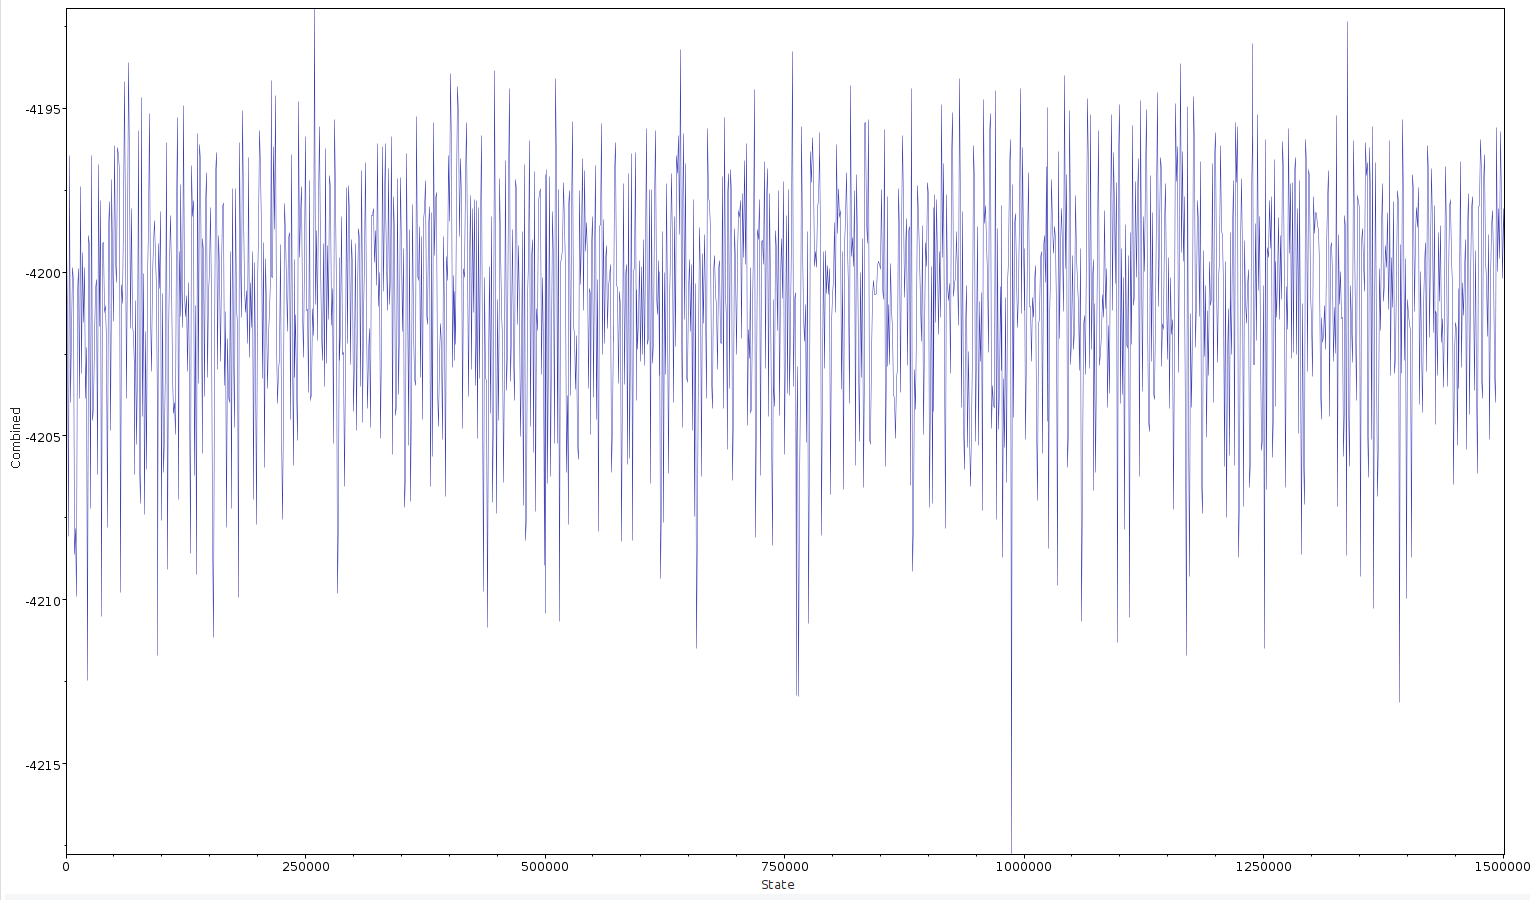
\includegraphics[width=0.5\textwidth]{../4/Phylogeny/trace.png}
		\caption[Convergence of lnL, BI analysis of Pn1.1317.]{Convergence of log likelihood of the cold chain, BI analysis of Pn1.1317 phylogeny.}
		\label{fig4_4}
	\end{wrapfigure}
	\FloatBarrier


	This analysis was run in the CIPRES Science Gateway portal. \cite{cipres} To verify if convergence was reached, the results were analyzed with Tracer, the effective sample size for all the parameters was higher than 200: the log likelihood of the
	cold chain (LnL: 1721; Fig \ref{fig4_4}), the log likelihood of the prior (LnPr: 1668) and the total tree length (TL: 1658). \cite{tracer}
	The resulting tree of the BI analysis can be seen in Fig. \ref{fig4_5} Based on this results, the sequence with PDB ID: \href{https://www.rcsb.org/structure/1KYW}{1KYW}, a Caffeic Acid/5-hydroxyferulic acid 3/5-O-methyltransferase from \textit{Medicago sativa} was selected to define the binding site for caffeic acid. It is part of the sister group of Pn1.1317 and had the most significant alignment E-value ($2\times10^{-180}$). 
	

	\FloatBarrier
	\begin{wrapfigure}[15]{l}{0.5\textwidth}
		\centering
		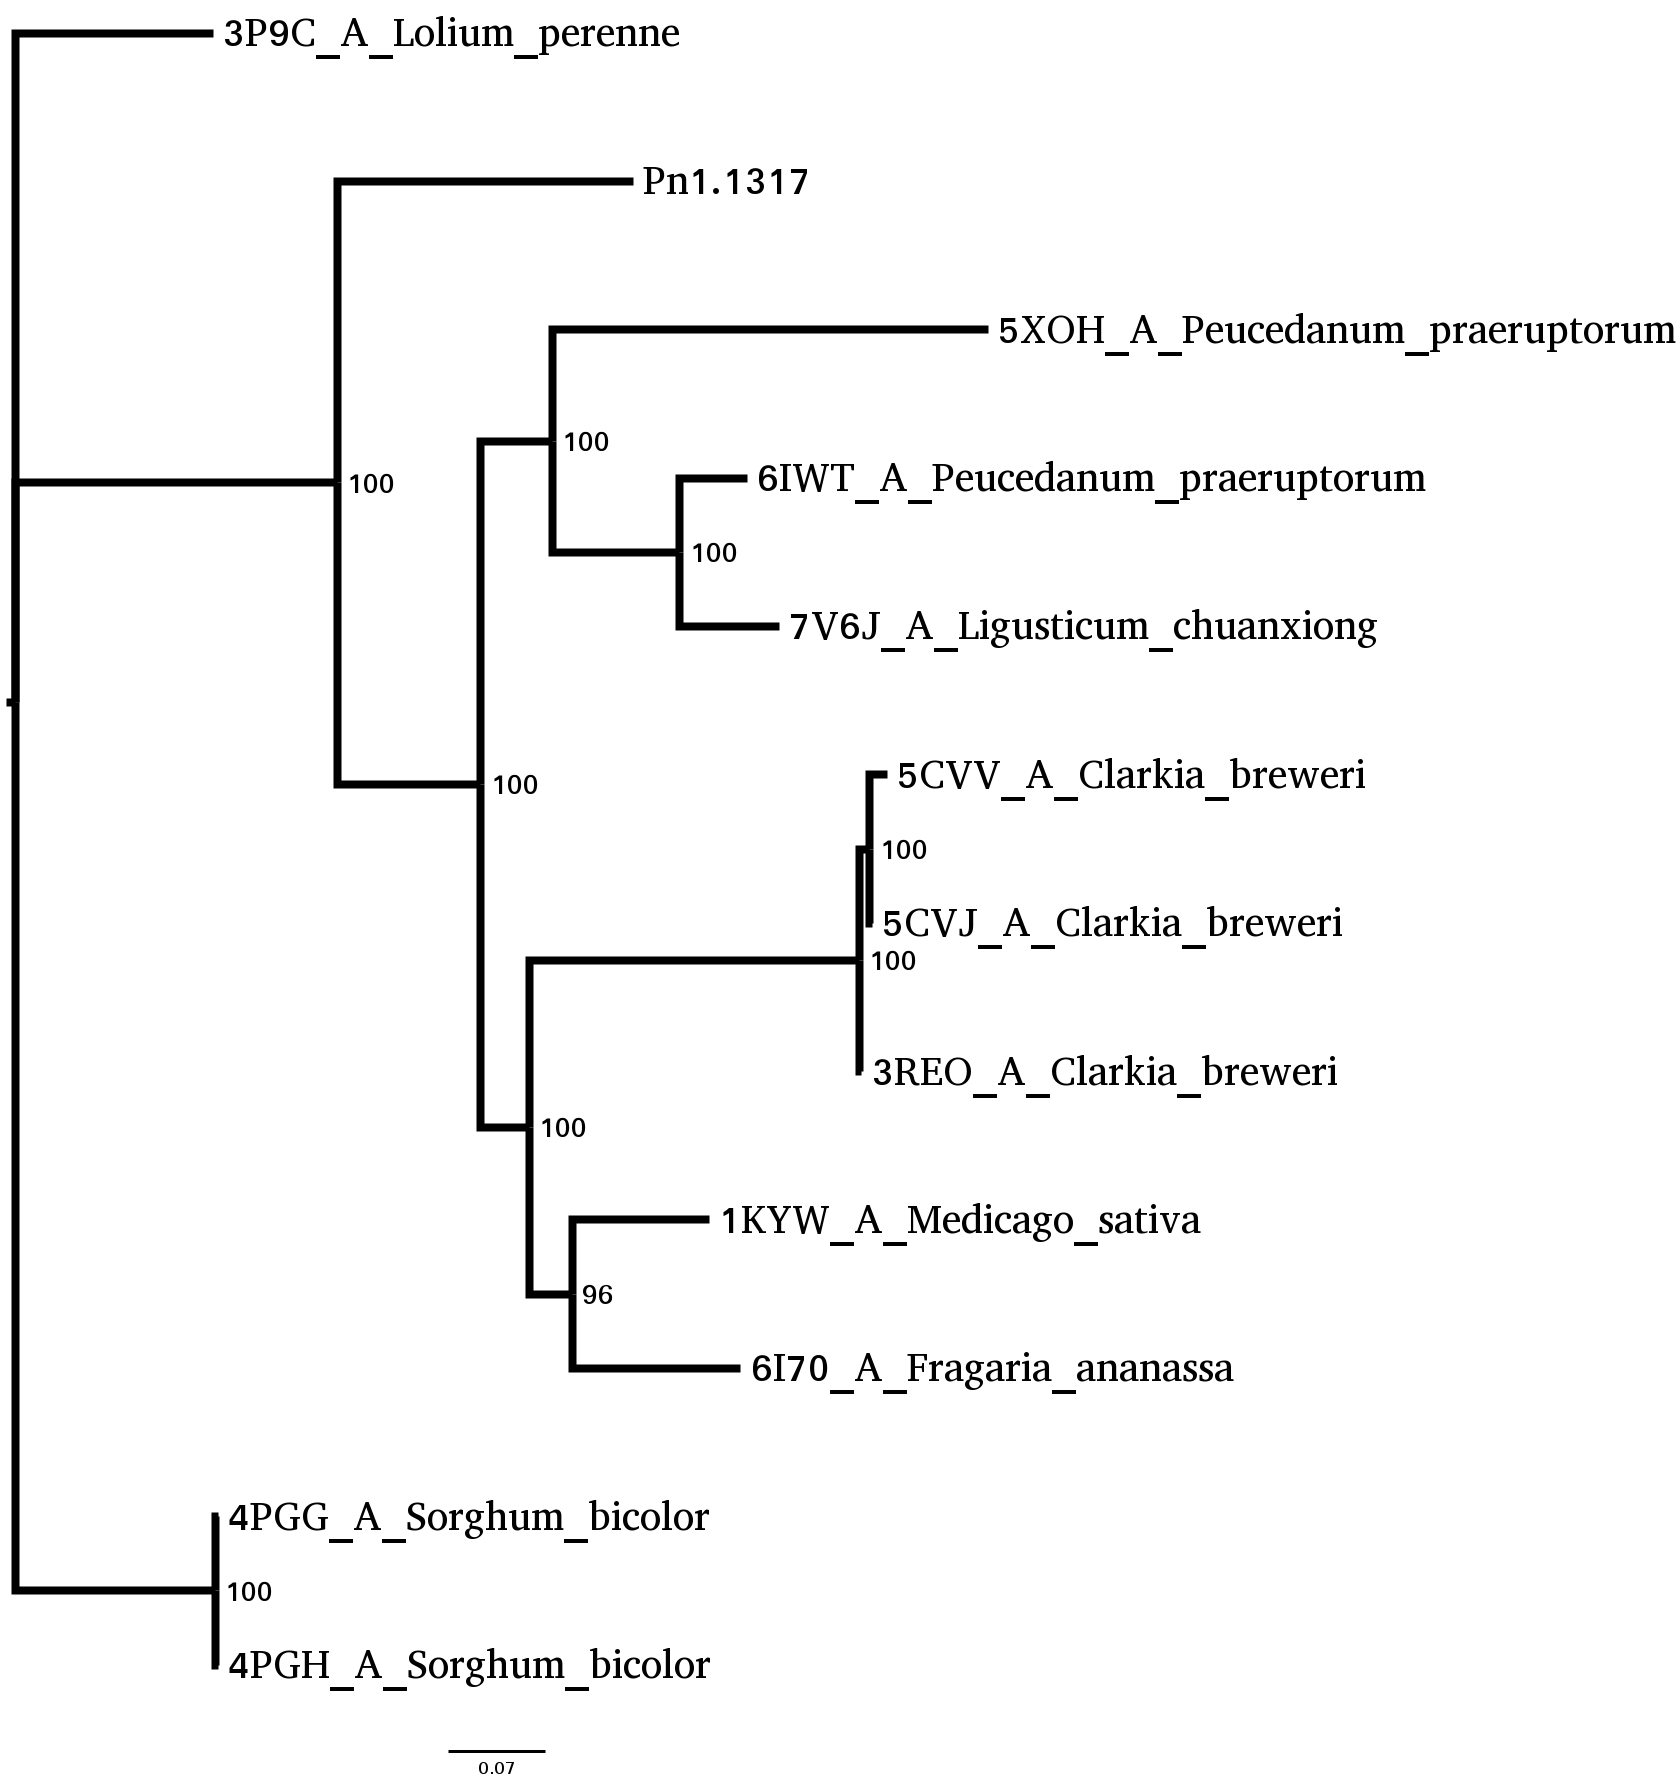
\includegraphics[width=0.5\textwidth-10pt]{../4/Phylogeny/tree.png}
		\caption{Phylogeny of Pn1.1317, Bayesian Inference.}
		\label{fig4_5}
	\end{wrapfigure}
	\FloatBarrier
	
	Based on the results obtained for this protein by \textcite{caff}, the interactions the substrate HFL (5-(3,3-dihydroxypropeny)-3-methoxy-benzene-1,2-diol) with 1KYW from the crystalographic structure (Fig. \ref{fig4_6}) and its homology with Pn1.1317 eleven aminoacid residues were selected as putative binding site for caffeic acid: Met 127, Leu 133, Ala 159, Phe 173, Met 177, Asp 267, Val 313, Ile 316, Met 317, His 320 and Asn 321.
	
	CASTp3 found the protein's pockets. \cite{castp} To perform an adequate docking of both the SAM molecule and the caffeic acid, a sequential docking workflow was used as described in \textcite{sequential} and in section \ref{ssec:Pn2.84}.
	
	\newpage
	
	\FloatBarrier
	\begin{wrapfigure}{r}{0.5\textwidth}
		\centering
		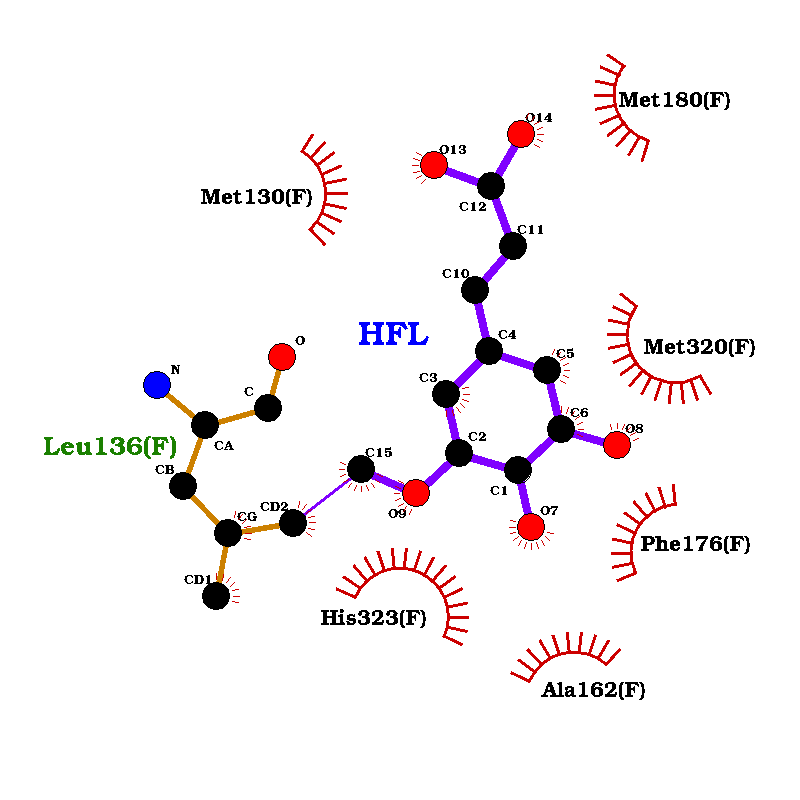
\includegraphics[width=0.5\textwidth]{../4/Phylogeny/hfl.png}
		\caption{Interactions between caffeic acid and 1KYW.}
		\label{fig4_6}
	\end{wrapfigure}
	\FloatBarrier
	
	\subsubsection{SAM}
	
	The first molecule docked was the SAM molecule, as a result of molecular docking with Vina, nine different conformations of the molecule in the protein were found, these results are shown in Table \ref{table4_1}. The docked positions of the protoporphyrin IX with Fe in the Pn2.84 structure interacted with different aminoacid residues of the protein (Fig. \ref{fig4_7}). Some of these aminoacids were found in the conserved domain for the SAM/SAH binding site of the enzyme, like Phe 160, Phe 173, Met 177, Ser 181, Gly 205, Gly 207, Asp 228, Leu 229, Val 232, Asp 248, Met 249, Lys 262, Trp 263, Ile 264, Asp 267 and Trp 268; the rest of the aminoacids were not marked as conserved in the heme binding site domain but were present in the pockets found by CASTp3: Asn 174, Ser 178, Gly 206, Ala 211, Phe 227 and Gly 247. In Fig. \ref{fig4_8} the SAM in its pocket is shown, the surface of the protein is colored based on its hydrophobicity using Kyte-Doolittle scale from lower (blue) to higher hydrophobicity (red).
	
	\begin{table}[h!]
		\centering
		\caption{Docking results of SAM with Pn1.1317}
		\label{table4_1}
		\begin{tabular}{cccc}
			\toprule
			\multirow{2}{*}{Mode} & Affinity & \multicolumn{2}{c}{Dist. from best mode}\\
			&  (kcal/mol) & RMSD l.b & RMSD u.b\\
			\midrule
			1 & -8.594   &       0   &       0\\
			2 & -8.476   &   1.118   &   1.323\\
			3 & -8.364   &   2.652   &   8.627\\
			4 &  -8.13   &   1.703   &   2.671\\
			5 & -8.113   &   2.585   &   8.519\\
			6 & -7.993   &   2.473   &    3.43\\
			7 & -7.778   &   2.394   &   3.229\\
			8 & -7.471   &   1.715   &   2.739\\
			9 & -7.239   &   3.722   &   8.452\\
			\bottomrule
			
		\end{tabular}
	\end{table}
	
	\FloatBarrier
	\begin{figure}[h!]
		\centering
		\begin{subfigure}[h!]{0.35\textwidth}
			\hspace{2cm}
			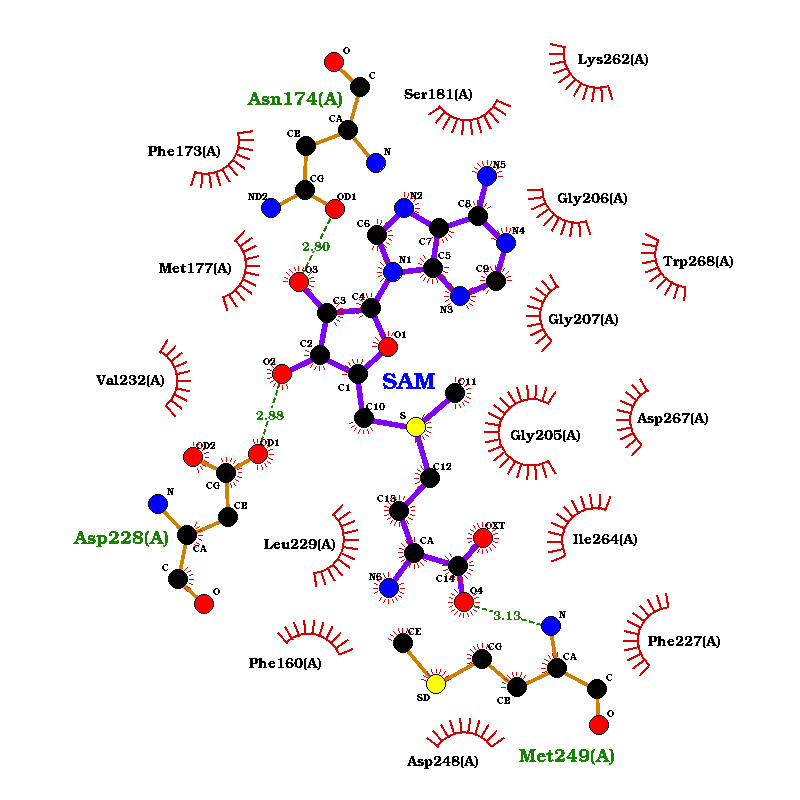
\includegraphics[width=\textwidth]{../4/Dock/best.png}
			\caption{}
		\end{subfigure}
		\hfill
		\begin{subfigure}[h!]{0.35\textwidth}
			\hspace{-2cm}
			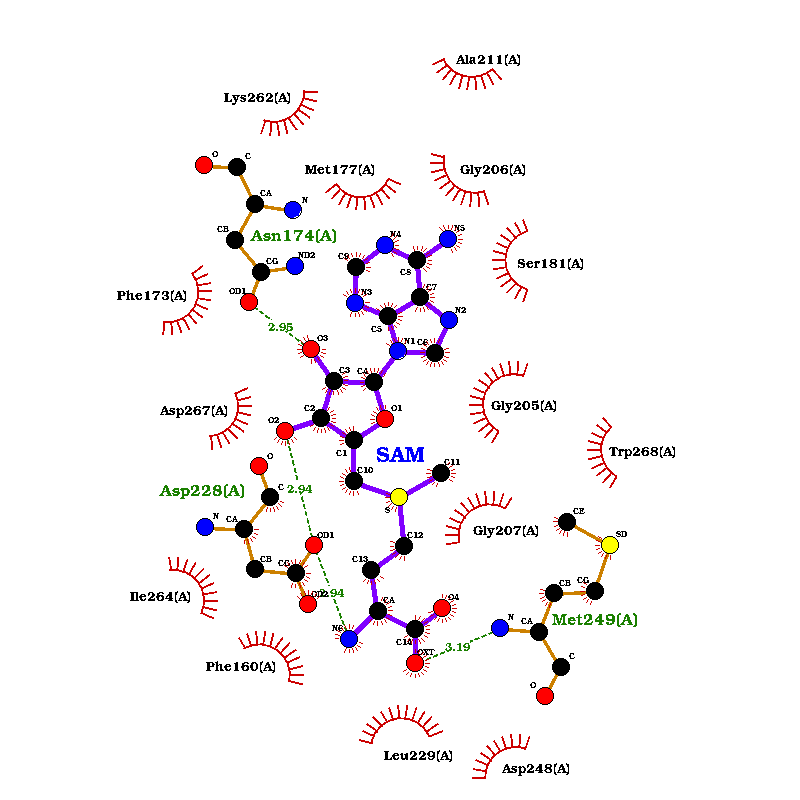
\includegraphics[width=\textwidth]{../4/Dock/best2.png}
			\caption{}
		\end{subfigure}
		\hfill
		\begin{subfigure}[h!]{0.35\textwidth}
			\hspace{2cm}
			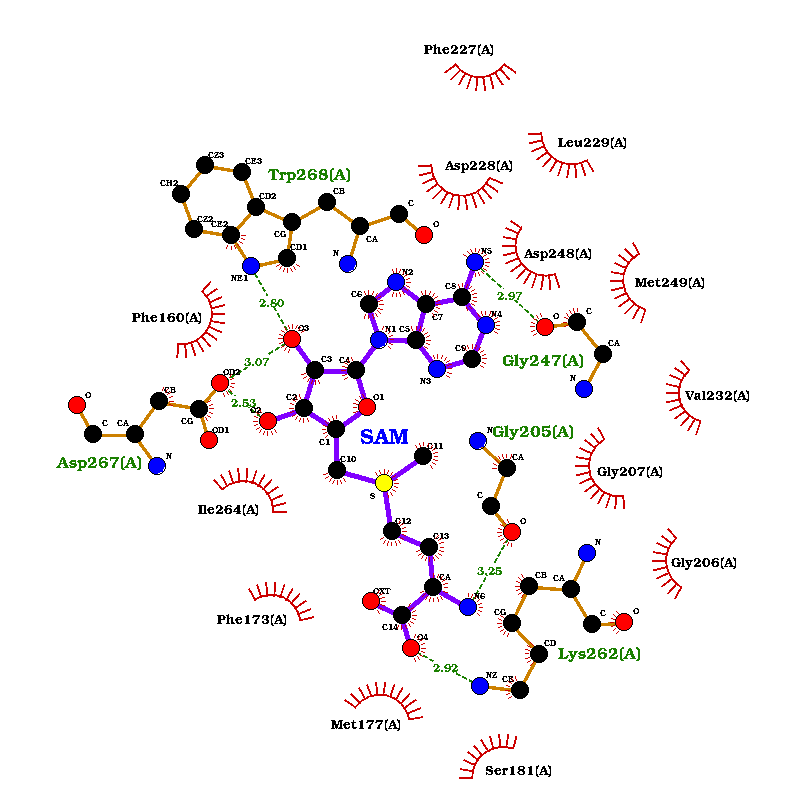
\includegraphics[width=\textwidth]{../4/Dock/best3.png}
			\caption{}
		\end{subfigure}
		\hfill
		\begin{subfigure}[h!]{0.35\textwidth}
			\hspace{-2cm}
			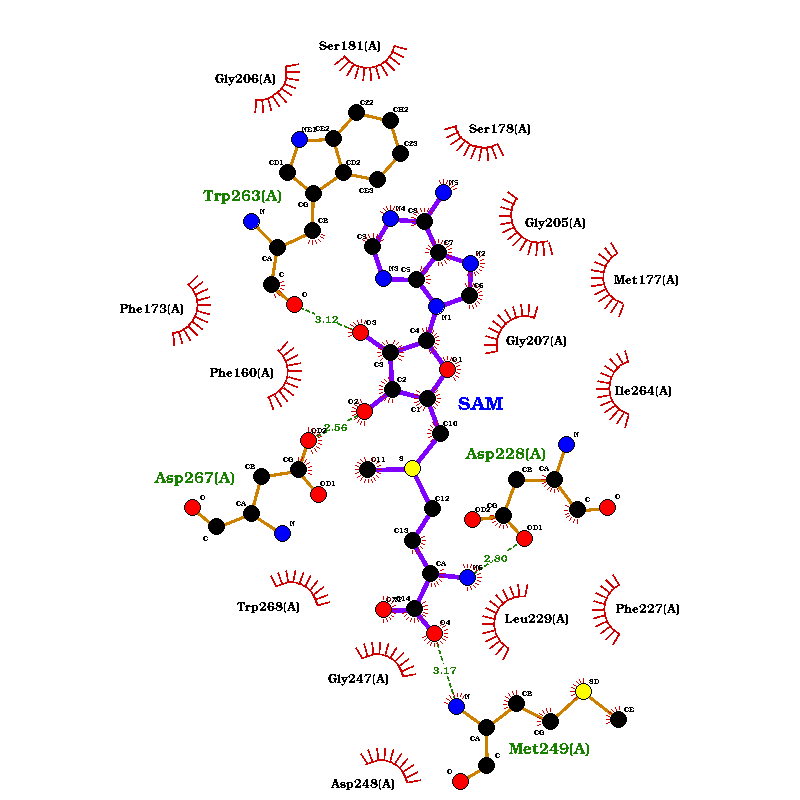
\includegraphics[width=\textwidth]{../4/Dock/best4.png}
			\caption{}
		\end{subfigure}
		\hfill
		\caption[Interactions between SAM and Pn1.1317.]{Interactions between SAM and Pn1.1317. Best four poses are shown in order a-d.}
		\label{fig4_7}
	\end{figure}
	\FloatBarrier
	
	\FloatBarrier
	\begin{figure}[h!]
		\centering
		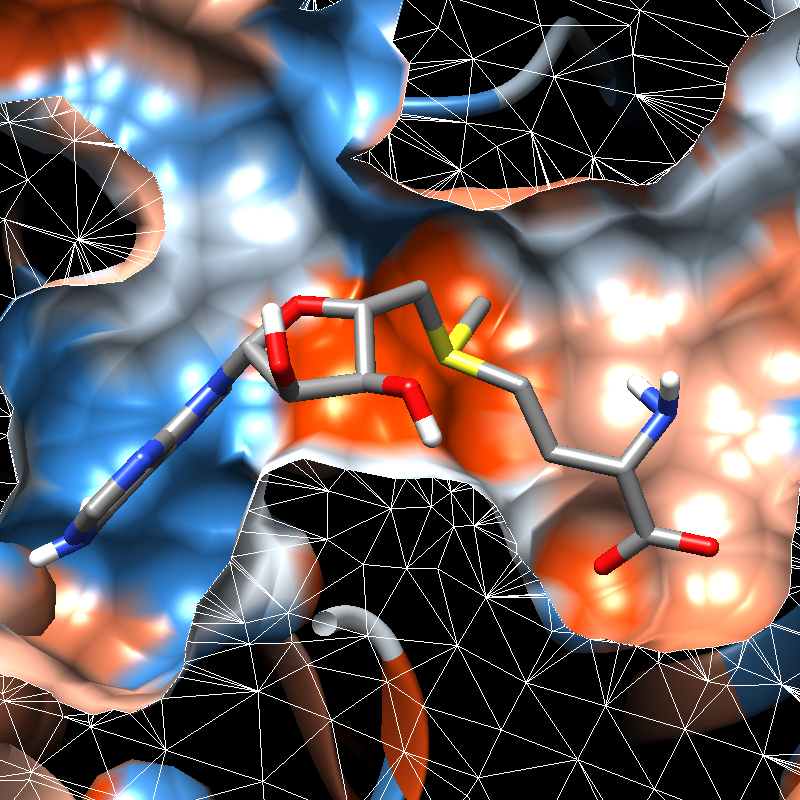
\includegraphics[width=0.4\textwidth]{../4/Dock/chimera.png}
		\caption{SAM in pocket of Pn1.1317.}
		\label{fig4_8}
	\end{figure}
	\FloatBarrier
	
	
	\subsubsection{Caffeic acid}
	
	With the Pn1.1317 protein and the best docked pose of SAM as a complex, molecular docking using Vina was carried out for caffeic acid resulting in nine different conformations, these results are shown in Table \ref{table4_2} The docked positions of the caffeic acid in the receptor structure interacted with different aminoacid residues of the protein (Fig. \ref{fig4_9}). Some of these aminoacids were found between the residues considered the active site of the enzyme and important for caffeic acid binding according to \textcite{caff}: the hydrophobic residues Met 127, Phe 173, Met 177 and Met 317 sequester the phenyl ring that presents the reactive hydroxyl group to SAM, the residues Asp 267 and Asn 321 form hydrogen bonds with 5-OH group, interactions with the residues Asn-128, Met 127, Met 177, Val 313, and Ile 316 are necessary to bind the propanoid tail;
	the rest of the aminoacids were not marked as conserved in the active site domain but were present in the pockets found by CASTp3: Met 21, Leu 124, Trp 263 and His 266. In Fig. \ref{fig4_10} the best docking pose of caffeic acid with SAM-Pn1.1317 in its pocket is shown, the surface of the protein is colored based on its hydrophobicity using Kyte-Doolittle scale from lower (blue) to higher hydrophobicity (red).
	

	\begin{table}[h]
		\centering
		\caption{Docking results of caffeic acid with SAM-Pn1.1317 complex}
		\label{table4_2}
		\begin{tabular}{cccc}
			\toprule
			\multirow{2}{*}{Mode} & Affinity & \multicolumn{2}{c}{Dist. from best mode}\\
			&  (kcal/mol) & RMSD l.b & RMSD u.b\\
			\midrule
			1 & -7.593   &   0.000   &   0.000\\
			2 & -7.298   &   0.769   &   1.874\\
			3 & -6.795   &   1.031   &   5.968\\
			4 & -6.067   &   1.058   &   5.939\\
			5 & -5.836   &   1.535   &   5.852\\
			6 & -5.691   &   2.752   &   5.559\\
			7 & -5.648   &   1.486   &   2.247\\
			8 & -5.393   &   2.771   &   5.849\\
			9 & -5.108   &   2.059   &   5.533\\
			\bottomrule
			
		\end{tabular}
	\end{table}
	
	\FloatBarrier
	\begin{figure}[h!]
		\centering
		\begin{subfigure}[h!]{0.35\textwidth}
			\hspace{2cm}
			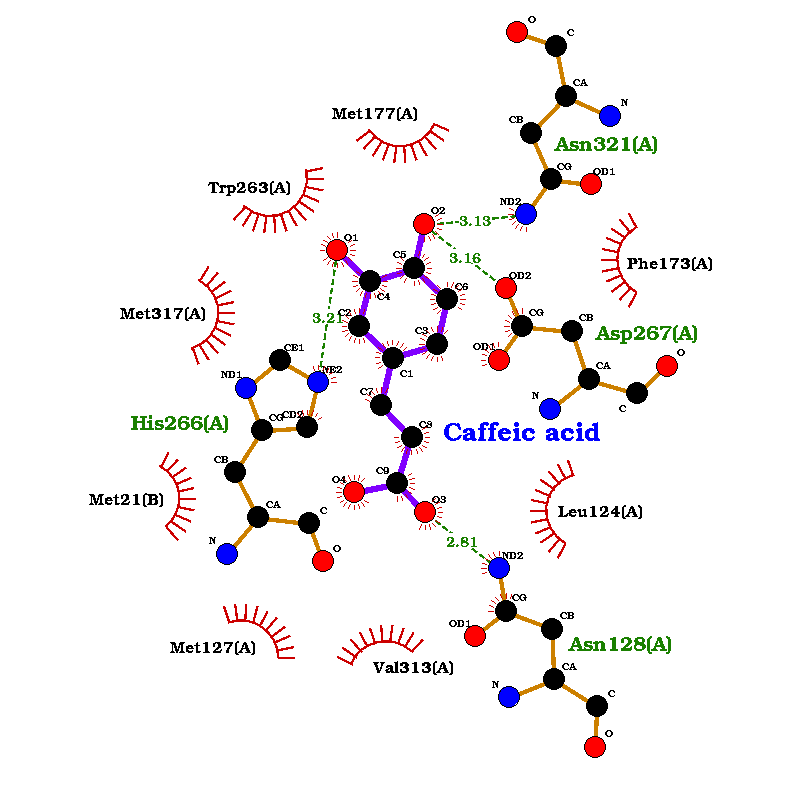
\includegraphics[width=\textwidth]{../4/Dock/Dock2/best.png}
			\caption{}
		\end{subfigure}
		\hfill
		\begin{subfigure}[h!]{0.35\textwidth}
			\hspace{-2cm}
			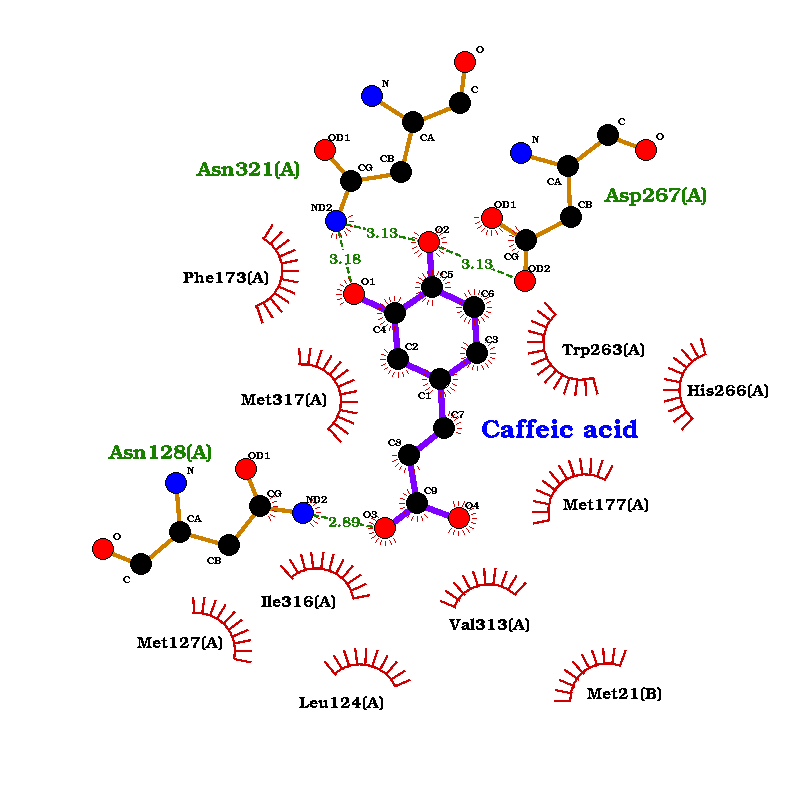
\includegraphics[width=\textwidth]{../4/Dock/Dock2/best2.png}
			\caption{}
		\end{subfigure}
		\hfill
		\begin{subfigure}[h!]{0.35\textwidth}
			\hspace{2cm}
			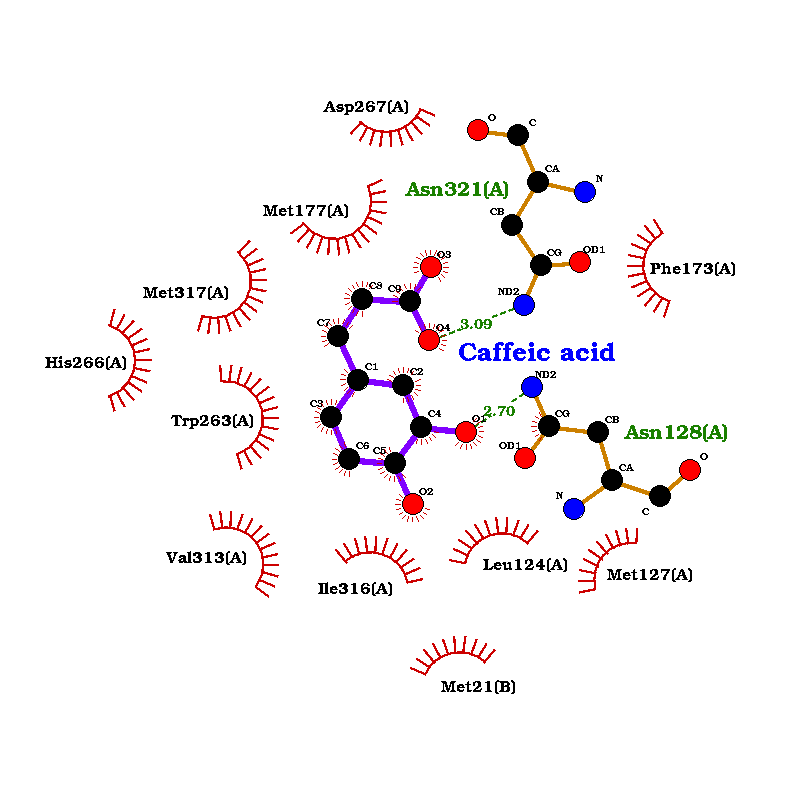
\includegraphics[width=\textwidth]{../4/Dock/Dock2/best3.png}
			\caption{}
		\end{subfigure}
		\hfill
		\begin{subfigure}[h!]{0.35\textwidth}
			\hspace{-2cm}
			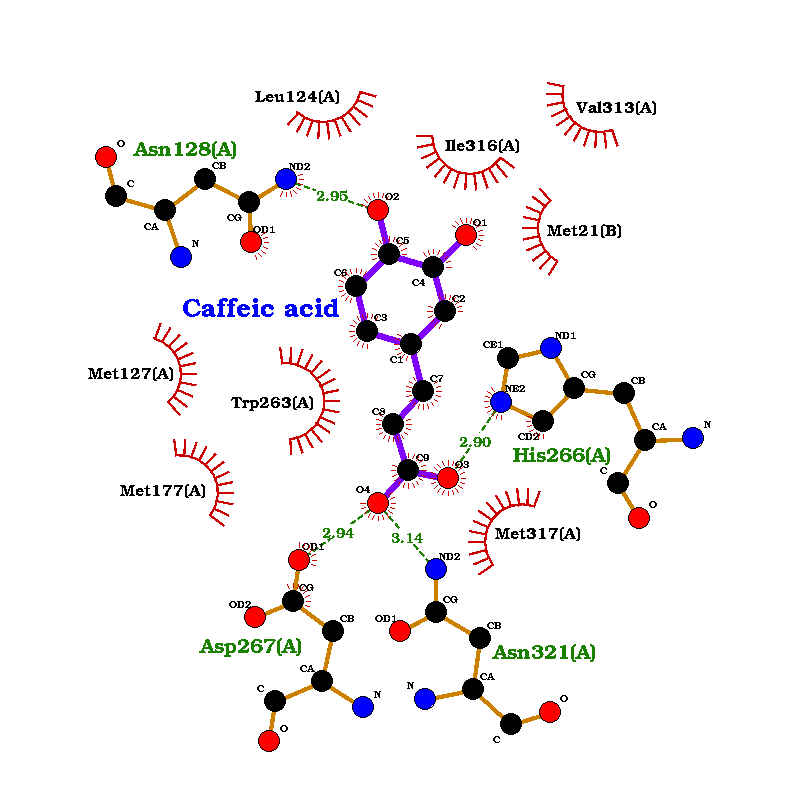
\includegraphics[width=\textwidth]{../4/Dock/Dock2/best4.png}
			\caption{}
		\end{subfigure}
		\hfill
		\caption[Interactions between caffeic acid and SAM-Pn1.1317 complex.]{Interactions between SAM and Pn1.1317. Best four poses are shown in order a-d.}
		\label{fig4_9}
	\end{figure}
	\FloatBarrier
	
	\FloatBarrier
	\begin{figure}[h!]
		\centering
		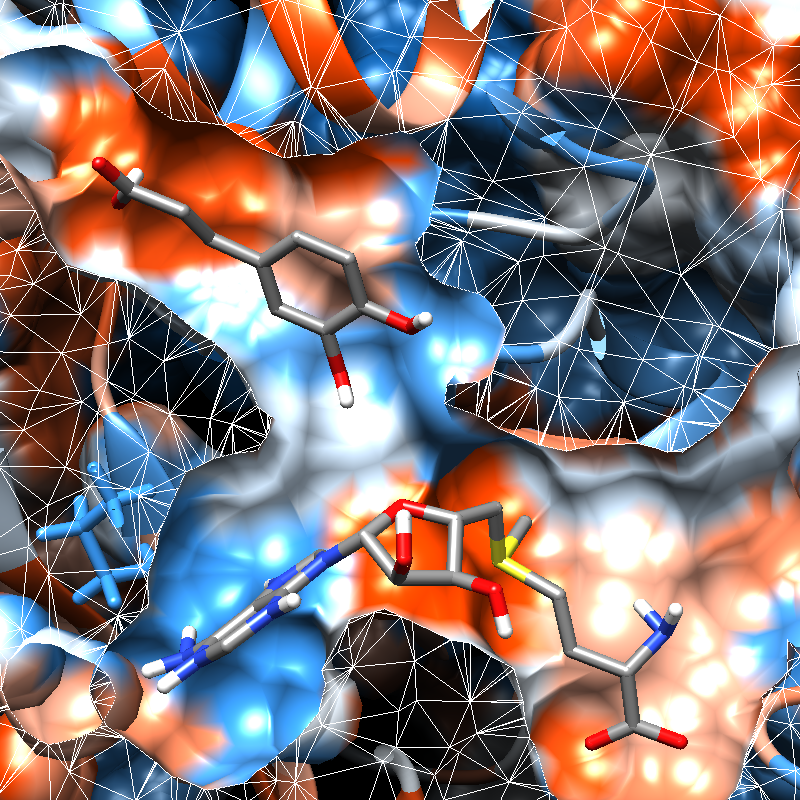
\includegraphics[width=0.4\textwidth]{../4/Dock/Dock2/chimera.png}
		\caption{Caffeic acid in pocket of SAM-Pn1.1317 complex.}
		\label{fig4_10}
	\end{figure}
	\FloatBarrier
	
	\newpage
	
	\subsection{Pn3.4770}
	
	The fifth reaction of the pathway (Eq. \ref{eq4}) is catalyzed by a protein similar to CYP719A37. The gene Pn3.4770 was selected as a candidate for enzyme 5 based on the fact that it has a 100\% identity to CYP719A37 (E-value $\approxeq 0$) with accession number: \href{https://www.ncbi.nlm.nih.gov/protein/QQS74306.1/}{QQS74306}. The protein CYP719A37 has a length of 511 aminoacid residues, but the gene Pn3.4770 codifies for 578 aminoacids; this indicates that maybe there is an alternative splicing process affecting the expression of this gene. A Blast result and the exon usage analysis showed that from the three exons present in gene Pn3.4770, only the first two exons were expressed (Fig \ref{fig5k_1}).
	
	\begin{equation}
	\schemestart
	\chemname{\footnotesize\chemfig{-[:270]O-[:210]-[:270](-[:330,,,1]OH)(%
-[:150,,,,draw=none]\mcfcringle{1.3})-[:210]-[:150]-[:90](-[:30]-[:330])%
-[:150]-[:210,,,,drh]-[:150](=[:90]O)-[:210,,,2]HO}
}{Ferulic acid}\arrow{->[ 5]}\chemname{\footnotesize\chemfig{O=[:90](-[:30,,,1]OH)-[:150]-[:210,,,,drh]-[:150]-[:210]-[:150](%
-[:30,,,,draw=none]\mcfcringle{1.3})-[:90](-[:30]-[:330]-[:270])-[:162]O%
-[:234]-[:306]O(-[:18])}
}{\vspace{-100pt}}
	\label{eq4}
	\schemestop
	\end{equation}\\
	
	\vspace{-50pt}\hspace{0.5\paperwidth-20pt}
	\begin{minipage}{0.3\paperwidth}
		\centering
		3,4-Methylenedioxy cinnamic acid
	\end{minipage}\\
	
	\FloatBarrier
	\begin{wrapfigure}{r}{0.5\textwidth}
		\centering
		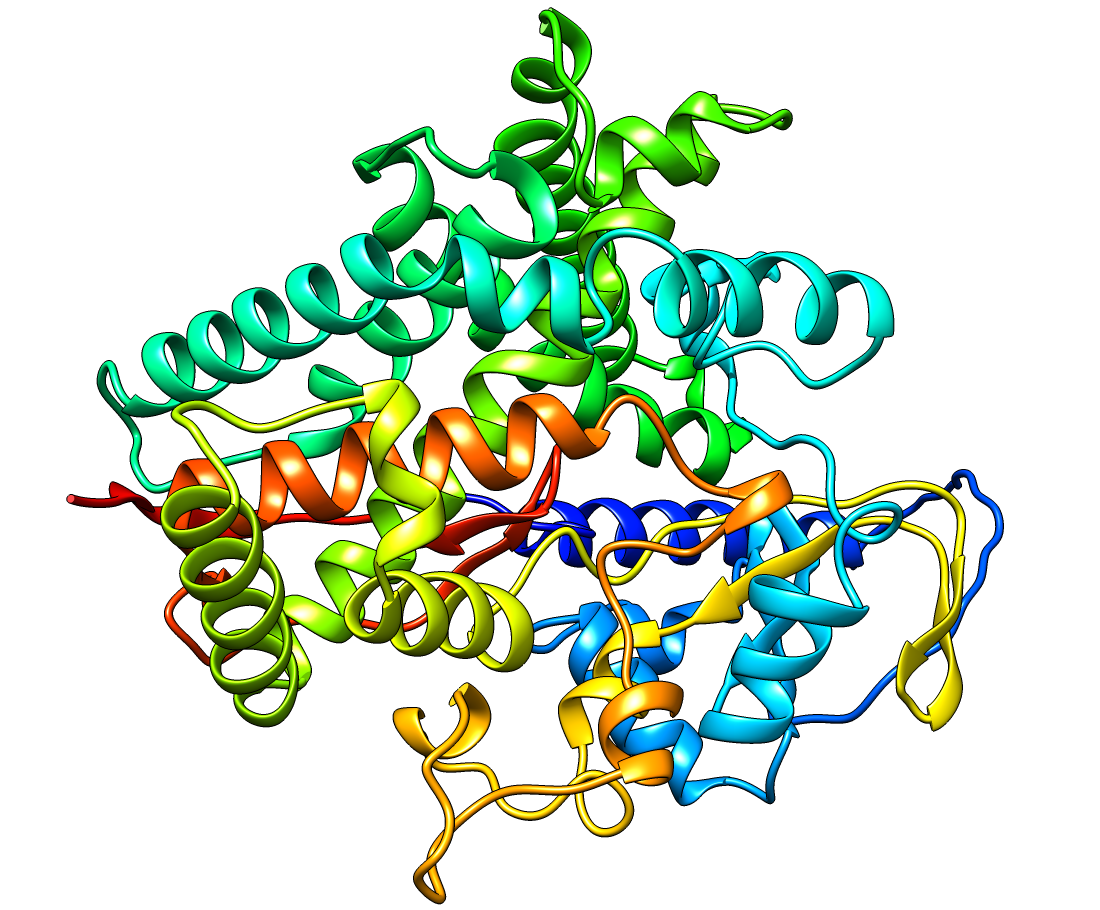
\includegraphics[width=0.5\textwidth]{../5/known/Minimize/model2.png}
		\caption{Pn3.4770 three-dimensional model.}
		\label{fig5k_2}
	\end{wrapfigure}
	\FloatBarrier
	
	Only the first two exons of the gene were considered when modeling the three-dimensional structure of the protein. The structure modeling was made by using an artificial intelligence based methodology, the algorithm used for the 3D structure prediction of the protein was AlphaFold2 using the ColabFold resource. \cite{alphafold,colabfold} ColabFold is a collaboratory space that allows users to perform three-dimensional structure prediction using AlphaFold2, AlphaFold2 multimer, MMseqs2 and HHsearch; this without having a super computer capable of running AlphaFold2 locally. The Local Distance Difference Test (lDDT) can be seen in Fig \ref{fig5k_3}, this is a well suited score to assess local model quality. \cite{lddt}
	
	The enzyme requires an heme molecule as a coenzyme for its correct catalytic activity; in this case the protoporphyrin IX containing Fe was selected based on the heme group present in the template for a ``SWISS-MODEL'' structure prediction that was made, the template was the CYP-450 17A1 protein from \textit{Danio rerio} with PDB ID: \href{https://www.rcsb.org/structure/6b82}{6b82}; this model was not selected because of the low sequence identity with Pn3.4770 (24.62\%). The ligand 3D conformer structure was obtained from PubChem with CID: \href{https://pubchem.ncbi.nlm.nih.gov/compound/445858}{445858}.
	
	\FloatBarrier
	\begin{figure}[h!]
		\centering
		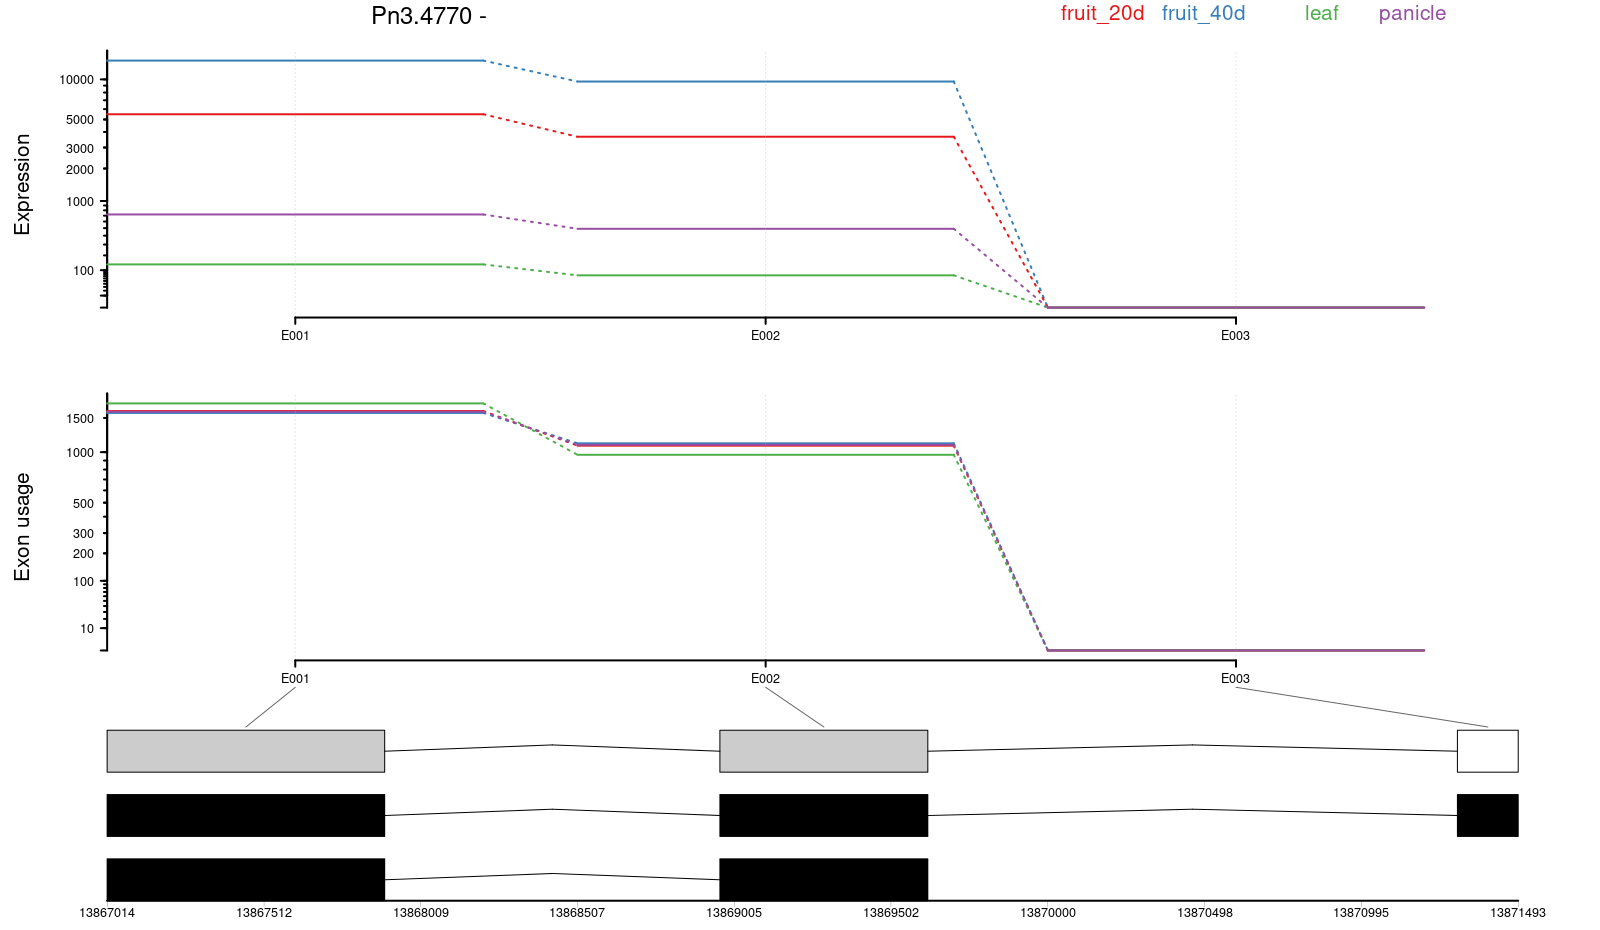
\includegraphics[width=\textwidth-50pt]{../5/known/Transcripts/7.png}
		\caption{Exon usage analysis of Pn3.4770.}
		\label{fig5k_1}
	\end{figure}
	\FloatBarrier
	
	\FloatBarrier
	\begin{figure}[h!]
		\centering
		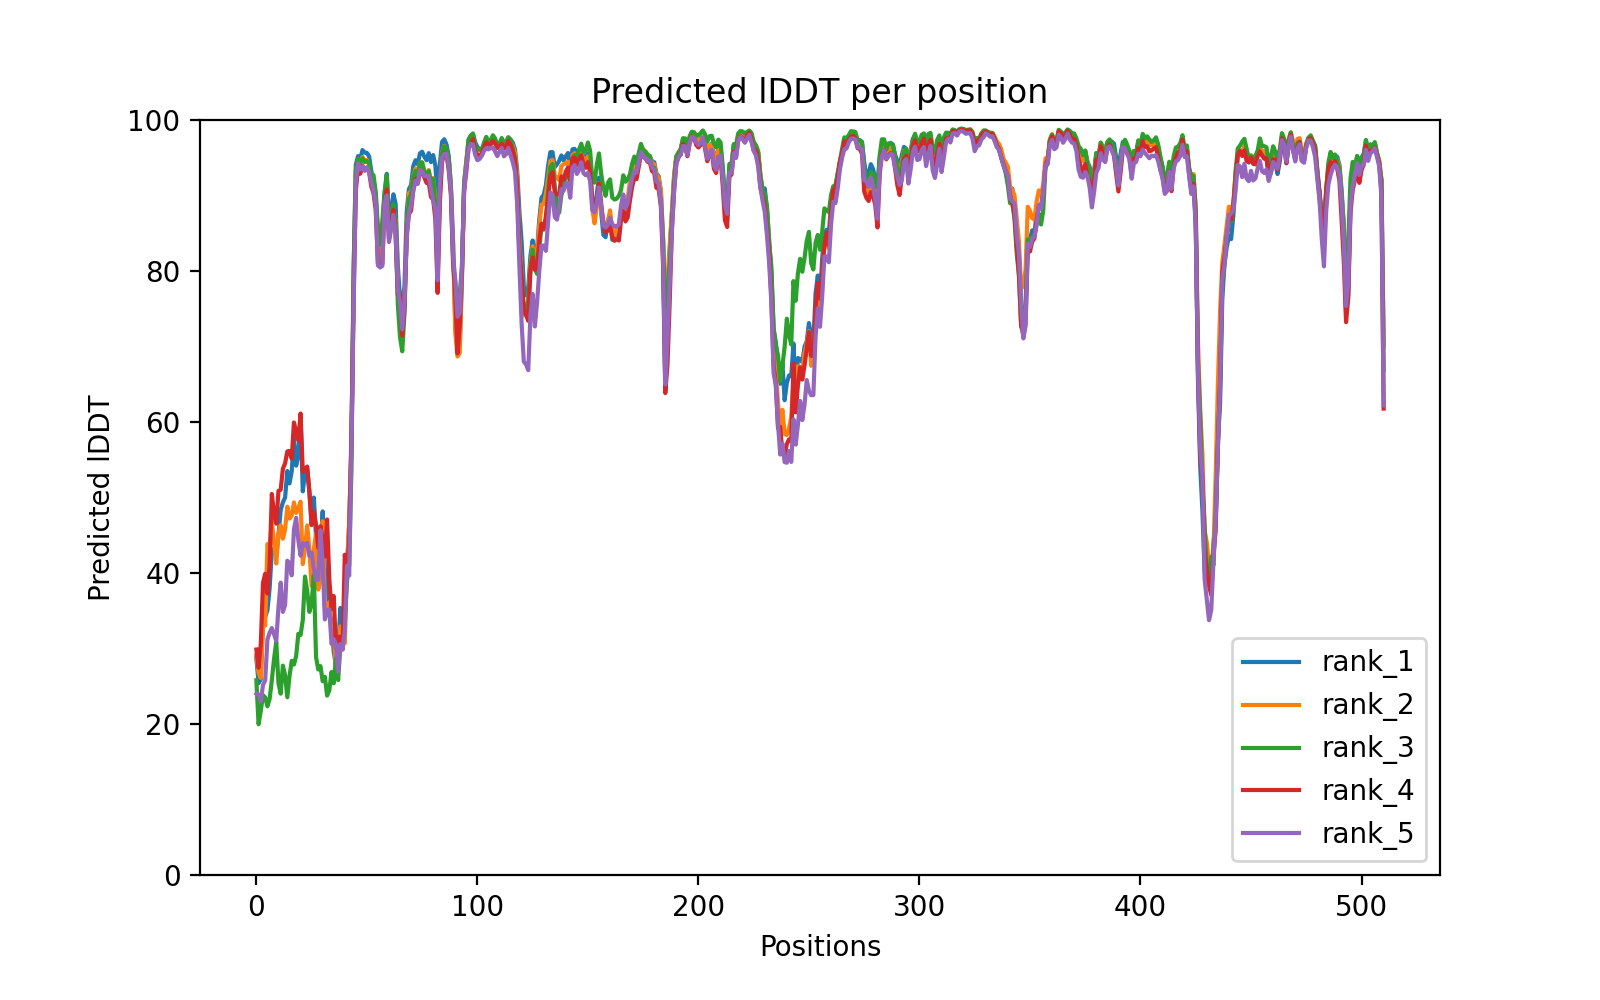
\includegraphics[width=\textwidth-50pt]{../5/known/AlphaFold2/Met_dioixi_ef326_plddt.png}
		\caption{lDDT values of Pn3.4770.}
		\label{fig5k_3}
	\end{figure}
	\FloatBarrier
	
	\newpage
	
	Before docking was performed the protein and the ligand were energy minimized. The protein structure was minimized using UCSF ChimeraX software \cite{chimera,chimera_2} and the steepest descent algorithm for 1000 steps with a step size of 0.02 \r{A}; the force field AMBER ff14SB was used for standar residues, for non standard residues the semi-empirical AM1-BCC model. \cite{am1_bcc,am1_bcc_2,am1_bcc_3} In the same way the ligand was energy minimized by using using the python library ``rdkit'' and the MMFF94 force field implemented within it. \cite{rdkit,rdkit_mmff}
	
	The preparation of the molecules for docking was made on AutoDockTools and Autodock Vina version 1.2.3 docked the protein and the ligand. \cite{adt,vina,vina_2} The grid box for the docking was selected based on the conserved domains found with the NCBI conserved domain search interface; we found the heme binding site and putative chemical substrate binding pocket conserved domains for cytochrome P450 family protein from the NCBI-Curated Domains database. \cite{cdd,cdd_2}  CASTp3 found the protein's pockets. \cite{castp} To perform an adequate docking of both the heme group and the ferulic acid molecule, a sequential docking workflow was used as described in \textcite{sequential} and in section \ref{ssec:Pn2.84}.
	
	It is important to mention that the sequence used in this methodology (CYP719A37) has been isolated by \textcite{methylenedioxy} and its activity has been tested with different substrates. Its original substrate is feruperic acid, which has a two carbon extension in comparison with ferulic acid; when using ferulic acid as a substrate the expected product (3,4-methylenedioxy cinnamic acid) could not be detected. This indicates that this enzyme could not be able to catalyze the reaction, despite this, the docking was performed in order to compare the results of this enzyme with the one that is proposed in this work that could perform the reaction. 
	
	\subsubsection{Protoporphyrin IX with Fe}
	
	The first molecule docked was the protoporphyrin IX with Fe, as a result of molecular docking with Vina, nine different conformations of the molecule in the protein were found, these results are shown in Table \ref{table5k_1}. The docked positions of the protoporphyrin IX with Fe in the Pn3.4770 structure interacted with different aminoacid residues of the protein (Fig. \ref{fig5k_4}). Some of these aminoacids were found in the conserved domain for the heme binding site of the enzyme, like Arg 119, Leu 156, Leu 206, Val 305, Leu 308, Gly 309, Ser 312, Thr 313, Ile 374, Ala 378, Val 379, His 381, Pro 447, Phe 448, Gly 449, Arg 453, Cys 455, Ala 456, Gly 457, Val 460 and Gly 461; the rest of the aminoacids were not marked as conserved in the heme binding site domain but were present in the pockets found by CASTp3: Val 135, Val 136, Leu 151, Glu 304, Thr 316, Met 369, Ala 375, Leu 404, Gln 464 and Val 465. In Fig. \ref{fig5k_5} the best docking pose of protoporphyrin IX with Fe with Pn3.4770 in its pocket is shown, the surface of the protein is colored based on its hydrophobicity using Kyte-Doolittle scale from lower (blue) to higher hydrophobicity (red).
	
	
	
	\begin{table}[h!]
		\centering
		\caption{Docking results of protoporphyrin IX (Fe) with Pn3.4770}
		\label{table5k_1}
		\begin{tabular}{cccc}
			\toprule
			\multirow{2}{*}{Mode} & Affinity & \multicolumn{2}{c}{Dist. from best mode}\\
			&  (kcal/mol) & RMSD l.b & RMSD u.b\\
			\midrule
			1 & -11.49   &       0   &       0\\
			2 & -11.04   &   2.227   &   6.083\\
			3 & -11.03   &   0.398   &   6.099\\
			4 & -10.48   &   2.164   &   6.827\\
			5 &  -9.85   &   2.162   &   6.136\\
			6 & -9.165   &    3.37   &    7.65\\
			7 & -8.075   &    3.45   &   7.137\\
			8 & -7.811   &   2.199   &   6.704\\
			9 & -7.369   &    1.92   &   6.276\\
			\bottomrule
			
		\end{tabular}
	\end{table}
	
	\FloatBarrier
	\begin{figure}[h!]
		\centering
		\begin{subfigure}[h!]{0.35\textwidth}
			\hspace{2cm}
			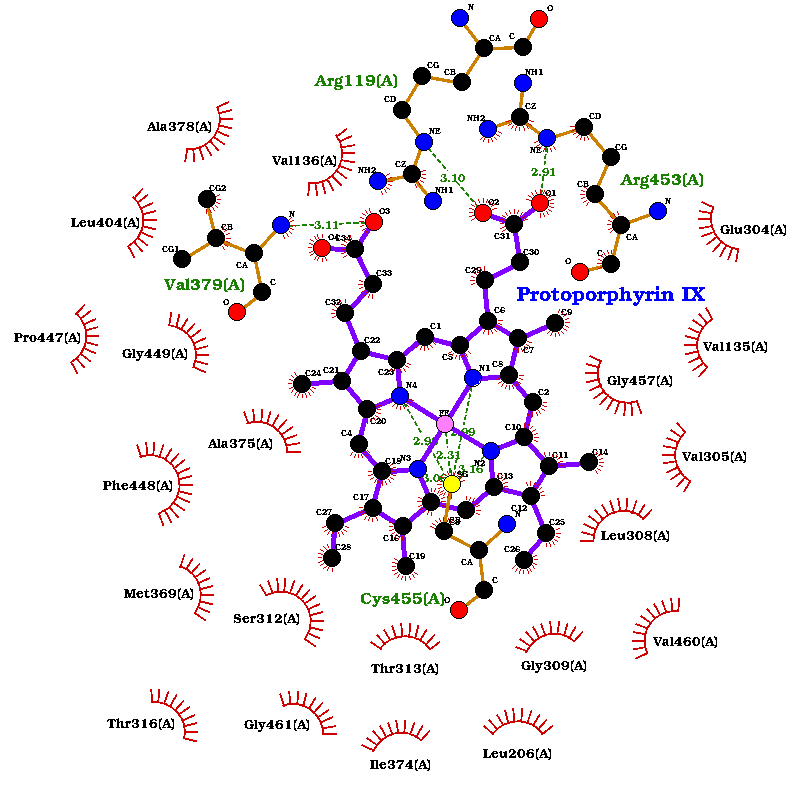
\includegraphics[width=\textwidth]{../5/known/Dock/best.png}
			\caption{}
		\end{subfigure}
		\hfill
		\begin{subfigure}[h!]{0.35\textwidth}
			\hspace{-2cm}
			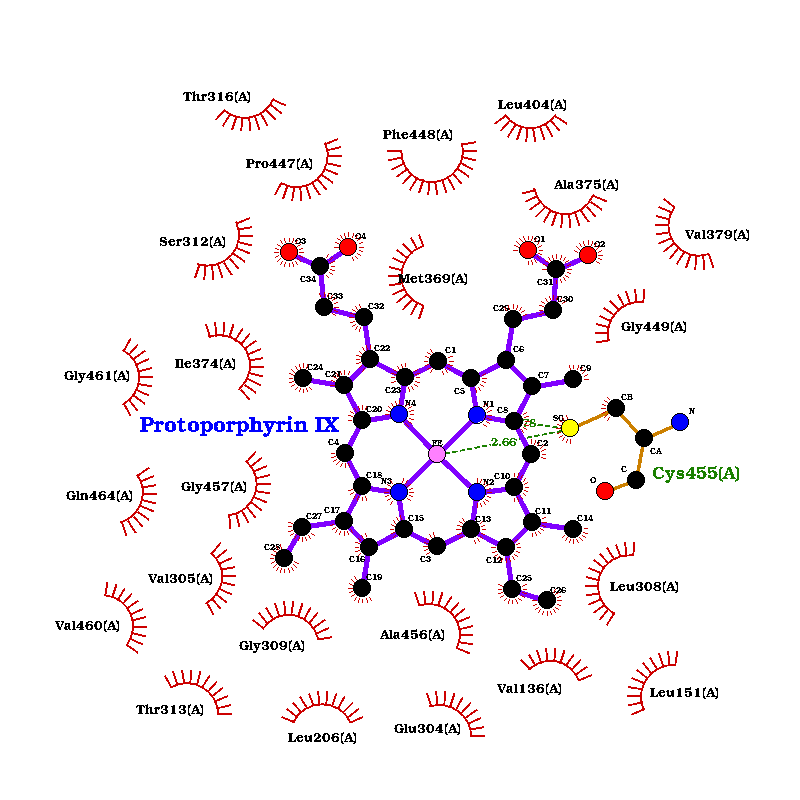
\includegraphics[width=\textwidth]{../5/known/Dock/best2.png}
			\caption{}
		\end{subfigure}
		\hfill
		\begin{subfigure}[h!]{0.35\textwidth}
			\hspace{2cm}
			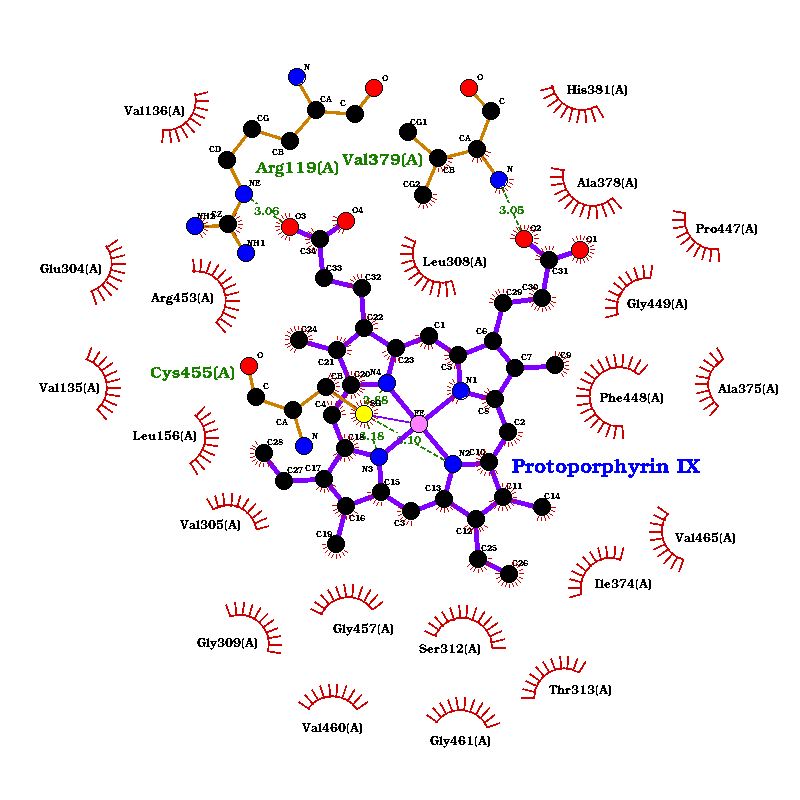
\includegraphics[width=\textwidth]{../5/known/Dock/best3.png}
			\caption{}
		\end{subfigure}
		\hfill
		\begin{subfigure}[h!]{0.35\textwidth}
			\hspace{-2cm}
			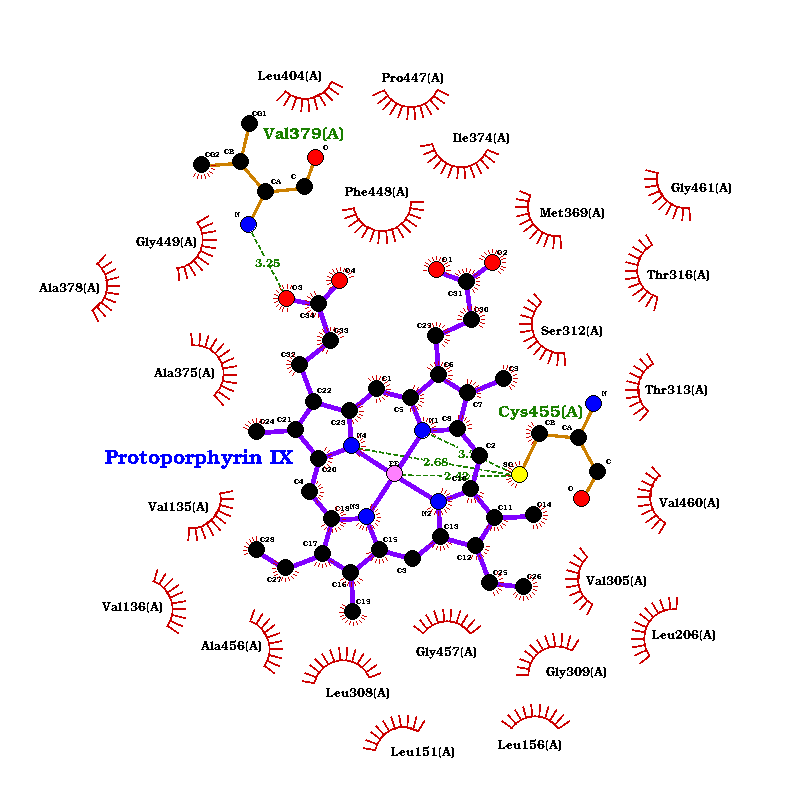
\includegraphics[width=\textwidth]{../5/known/Dock/best4.png}
			\caption{}
		\end{subfigure}
		\hfill
		\caption[Interactions between protoporphyrin IX with Fe and Pn3.4770.]{Interactions between protoporphyrin IX with Fe and Pn3.4770. Best four poses are shown in order a-d.}
		\label{fig5k_4}
	\end{figure}
	\FloatBarrier
	
	\FloatBarrier
	\begin{figure}[h!]
		\centering
		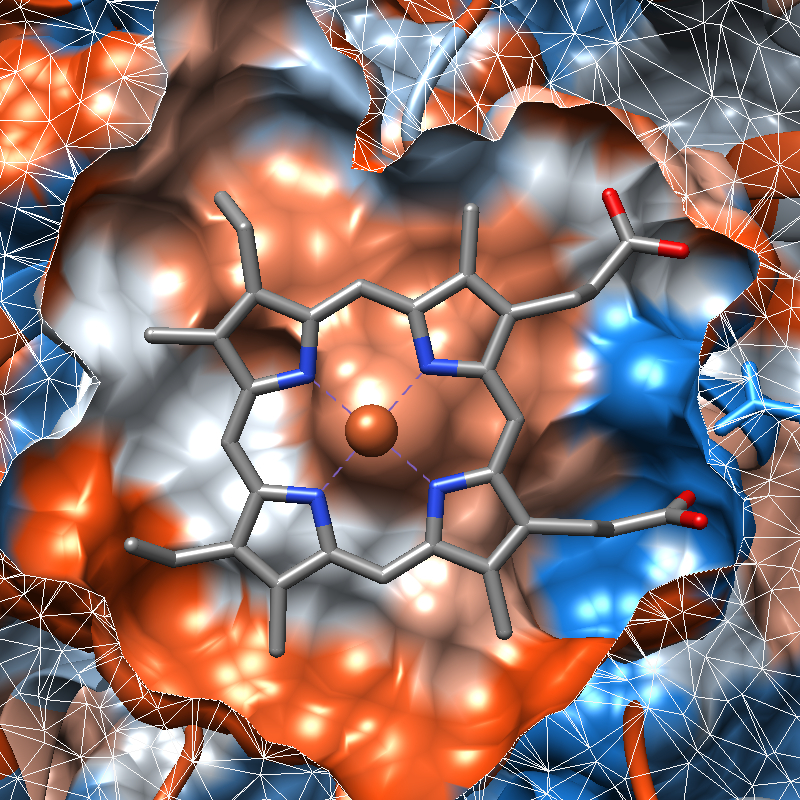
\includegraphics[width=0.4\textwidth]{../5/known/Dock/chimera.png}
		\caption{Protoporphyrin IX with Fe in pocket of Pn3.4770.}
		\label{fig5k_5}
	\end{figure}
	\FloatBarrier
	
	\subsubsection{Ferulic acid}
	
	\begin{wraptable}{r}{0.5\textwidth}
		\centering
		\caption{Docking results of ferulic acid with protoporphyrin IX-Pn3.4770 complex}
		\label{table5k_2}
		\begin{tabular}{cccc}
			\toprule
			\multirow{2}{*}{Mode} & Affinity & \multicolumn{2}{c}{Dist. from best mode}\\
			&  (kcal/mol) & RMSD l.b & RMSD u.b\\
			\midrule
			1 & -6.166   &       0   &       0\\
			2 & -5.987   &   2.709   &   5.073\\
			3 & -5.888   &   3.896   &   5.423\\
			4 & -5.841   &    2.87   &   4.927\\
			5 & -5.739   &   2.885   &   6.541\\
			6 & -5.563   &   2.609   &   5.194\\
			7 & -5.491   &     3.6   &   5.481\\
			8 & -5.302   &   2.348   &   3.964\\
			9 &  15.53   &   1.108   &   2.438\\
			\bottomrule
			
		\end{tabular}
	\end{wraptable}
	
	With the Pn3.4770 protein and the best docked pose of protoporphyrin IX with Fe as a complex, molecular docking using Vina was carried out for ferulic acid resulting in nine different conformations, these results are shown in Table \ref{table5k_2} The docked positions of the ferulic acid in the receptor structure interacted with different aminoacid residues of the protein (Fig. \ref{fig5k_6}). Some of these aminoacids were found in the conserved domain for the active site of the enzyme, like Leu 307, Leu 308 and Val 379; the rest of the aminoacids were not marked as conserved in the active site domain but were present in the pockets found by CASTp3: Leu 121, Phe 128, Asn 129, Val 136, Arg 239, Ser 312, Pro 380, Met 493 and Phe 495. In Fig. \ref{fig5k_7} the best docking pose of ferulic acid with protoporphyrin IX with Fe-Pn1.1317 complex in its pocket is shown, the surface of the protein is colored based on its hydrophobicity using Kyte-Doolittle scale from lower (blue) to higher hydrophobicity (red). The results show interactions between the ferulic acid and the Fe atom of protoporphyrin IX, but this interaction occurs in the propanoid tail instead of the 4-hydroxy-3-methoxyphenyl region.
	


	\FloatBarrier
	\begin{figure}[h!]
		\centering
		\begin{subfigure}[h!]{0.35\textwidth}
			\hspace{2cm}
			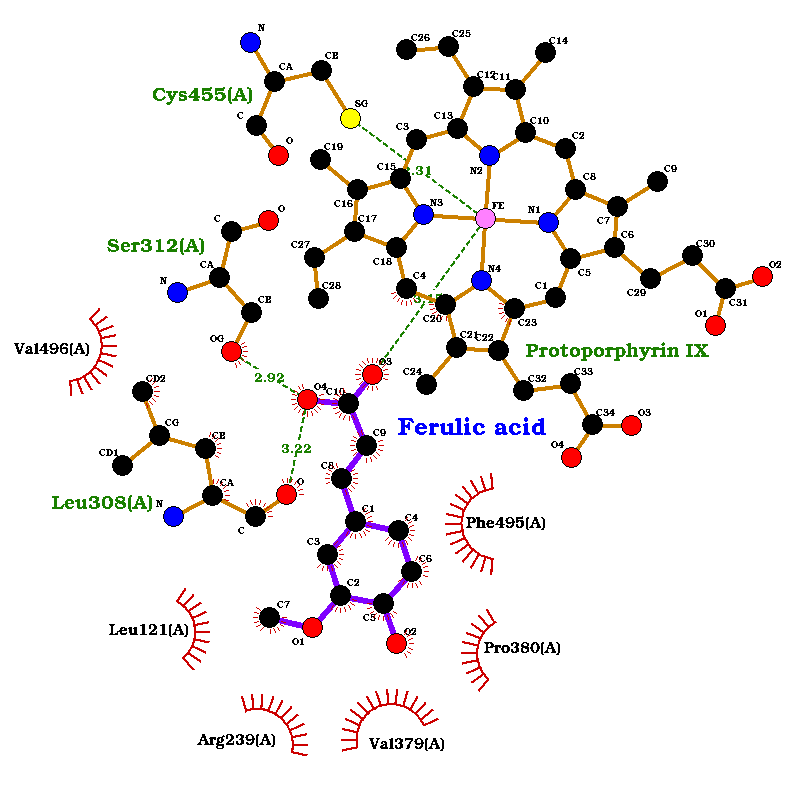
\includegraphics[width=\textwidth]{../5/known/Dock/Dock2/best.png}
			\caption{}
		\end{subfigure}
		\hfill
		\begin{subfigure}[h!]{0.35\textwidth}
			\hspace{-2cm}
			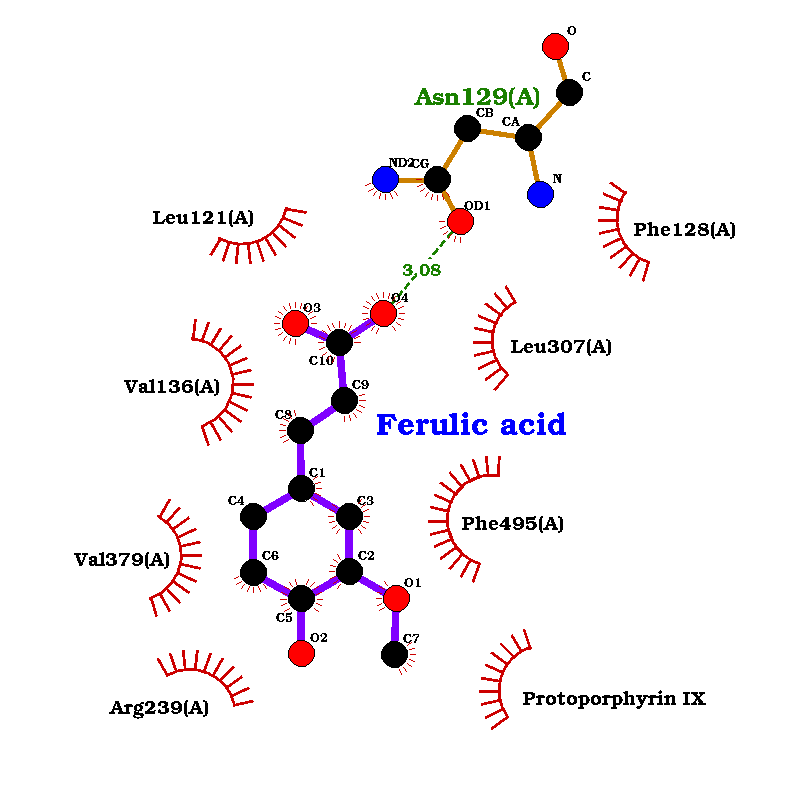
\includegraphics[width=\textwidth]{../5/known/Dock/Dock2/best2.png}
			\caption{}
		\end{subfigure}
		\hfill
		\begin{subfigure}[h!]{0.35\textwidth}
			\hspace{2cm}
			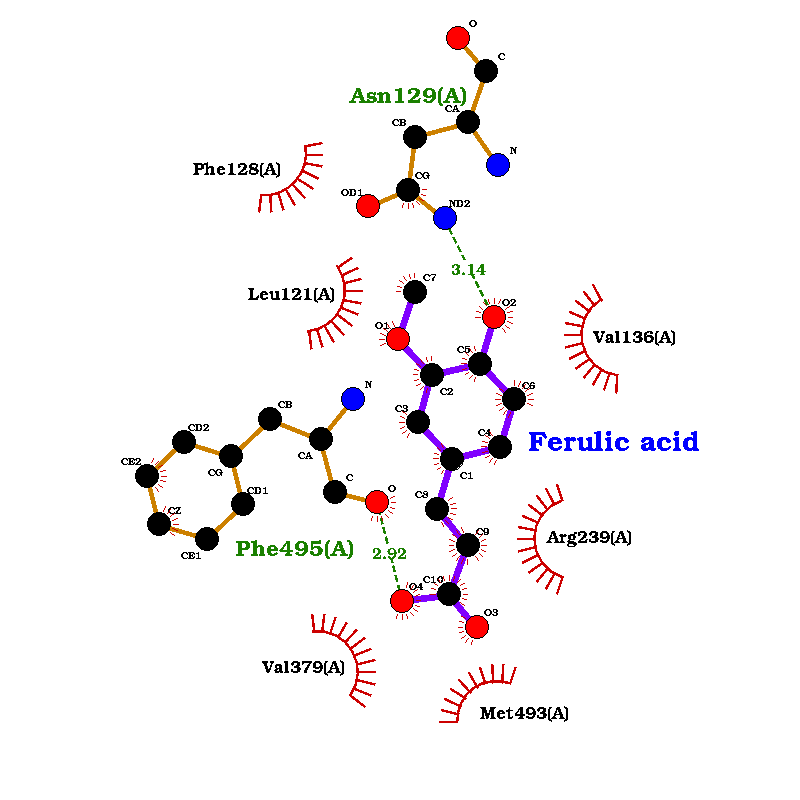
\includegraphics[width=\textwidth]{../5/known/Dock/Dock2/best3.png}
			\caption{}
		\end{subfigure}
		\hfill
		\begin{subfigure}[h!]{0.35\textwidth}
			\hspace{-2cm}
			\includegraphics[width=\textwidth]{../5/known/Dock/Dock2/best4.png}
			\caption{}
		\end{subfigure}
		\hfill
		\caption[Interactions between ferulic acid and protoporphyrin IX-Pn3.4770 complex.]{Interactions of ferulic acid with protoporphyrin IX-Pn3.4770 complex. Best four poses are shown in order a-d.}
		\label{fig5k_6}
	\end{figure}
	\FloatBarrier
	
	\FloatBarrier
	\begin{figure}[h!]
		\centering
		\includegraphics[width=0.4\textwidth]{../5/known/Dock/Dock2/chimera.png}
		\caption{Ferulic acid in pocket of protoporphyrin IX-Pn3.4770 complex.}
		\label{fig5k_7}
	\end{figure}
	\FloatBarrier
	
	\subsection{Pn7.1626}
	
	The fifth reaction of the pathway (Eq. \ref{eq4}) is catalyzed by a protein similar to CYP719A37. The gene Pn7.1626 was selected as a candidate for enzyme 5 based on the fact that it has the highest identity (76.908\%) to CYP719A37 from all other proteins in \textit{Piper nigrum} genome (E-value $\approxeq 0$). With the exon usage analysis no relevant results were found.
	
	\FloatBarrier
	\begin{wrapfigure}{r}{0.5\textwidth}
		\centering
		\includegraphics[width=0.5\textwidth]{../5/propose/Minimize/model2.png}
		\caption{Pn7.1626 three-dimensional model.}
		\label{fig5p_1}
	\end{wrapfigure}
	\FloatBarrier
	
	The two exons of the gene were considered when modeling the three-dimensional structure of the protein. The structure modeling was made by using an artificial intelligence based methodology, the algorithm used for the 3D structure prediction of the protein was AlphaFold2 using the ColabFold resource. \cite{alphafold,colabfold} The Local Distance Difference Test (lDDT) can be seen in Fig \ref{fig5p_2}, this is a well suited score to assess local model quality. \cite{lddt}
	
	The enzyme requires an heme molecule as a coenzyme for its correct catalytic activity; in this case the protoporphyrin IX containing Fe was selected based on the heme group present in the template for a ``SWISS-MODEL'' structure prediction that was made, the template was the CYP-450 17A1 protein from \textit{Danio rerio} with PDB ID: \href{https://www.rcsb.org/structure/6b82}{6b82}; this model was not selected because of the low sequence identity with Pn7.1626 (24.01\%). The ligand 3D conformer structure was obtained from PubChem with CID: \href{https://pubchem.ncbi.nlm.nih.gov/compound/445858}{445858}.
	
	Before docking was performed the protein and the ligand were energy minimized. The protein structure was minimized using UCSF ChimeraX software \cite{chimera,chimera_2} and the steepest descent algorithm for 1000 steps with a step size of 0.02 \r{A}; the force field AMBER ff14SB was used for standar residues, for non standard residues the semi-empirical AM1-BCC model. \cite{am1_bcc,am1_bcc_2,am1_bcc_3} In the same way the ligand was energy minimized by using using the python library ``rdkit'' and the MMFF94 force field implemented within it. \cite{rdkit,rdkit_mmff}
	
	The preparation of the molecules for docking was made on AutoDockTools and Autodock Vina version 1.2.3 docked the protein and the ligand. \cite{adt,vina,vina_2} The grid box for the docking was selected based on the conserved domains found with the NCBI conserved domain search interface; we found the heme binding site and putative chemical substrate binding pocket conserved domains for cytochrome P450 family protein from the NCBI-Curated Domains database. \cite{cdd,cdd_2}  CASTp3 found the protein's pockets. \cite{castp} To perform an adequate docking of both the heme group and the ferulic acid molecule, a sequential docking workflow was used as described in \textcite{sequential} and in section \ref{ssec:Pn2.84}.
	
	\FloatBarrier
	\begin{figure}
		\centering
		\includegraphics[width=\textwidth-50pt]{../5/propose/AlphaFold2/test_c0c6c_plddt.png}
		\caption{lDDT values of Pn7.1626.}
		\label{fig5p_2}
	\end{figure}
	\FloatBarrier
	
	
	\subsubsection{Protoporphyrin IX with Fe}
	
	The first molecule docked was the protoporphyrin IX with Fe, as a result of molecular docking with Vina, nine different conformations of the molecule in the protein were found, these results are shown in Table \ref{table5p_1}. The docked positions of the protoporphyrin IX with Fe in the Pn7.1626 structure interacted with different aminoacid residues of the protein (Fig. \ref{fig5p_3}). Some of these aminoacids were found in the conserved domain for the heme binding site of the enzyme, like Arg 111, Leu 148, Ile 197, Leu 296, Leu 299, Gly 300, Ser 303, Ser 304, Ile 365, Ala 369, Val 370, His 372, Pro 437, Phe 438, Gly 439, Arg 443, Cys 445, Ala 446, Gly 447, Val 450 and Gly 451; the rest of the aminoacids were not marked as conserved in the heme binding site domain but were present in the pockets found by CASTp3: Val 127, Ser 128, Leu 143, Glu 295, Thr 307, Met 360, Ala 366, Gln 454 and Ile 455. In Fig. \ref{fig5p_4} the best docking pose of protoporphyrin IX with Fe with Pn7.1626 in its pocket is shown, the surface of the protein is colored based on its hydrophobicity using Kyte-Doolittle scale from lower (blue) to higher hydrophobicity (red).
	
	
	
	\begin{table}[h!]
		\centering
		\caption{Docking results of protoporphyrin IX (Fe) with Pn7.1626}
		\label{table5p_1}
		\begin{tabular}{cccc}
			\toprule
			\multirow{2}{*}{Mode} & Affinity & \multicolumn{2}{c}{Dist. from best mode}\\
			&  (kcal/mol) & RMSD l.b & RMSD u.b\\
			\midrule
			1 &  -10.9   &       0   &       0\\
			2 & -10.63   &   1.916   &   6.174\\
			3 & -9.581   &   1.083   &   6.052\\
			4 & -9.251   &   2.084   &   5.954\\
			5 & -8.904   &   3.491   &   7.912\\
			6 & -8.866   &   4.112   &   7.679\\
			7 &  -8.81   &   3.957   &   9.337\\
			8 &  -8.21   &   1.608   &   5.955\\
			9 & -6.538   &   4.191   &   9.715\\
			\bottomrule
			
		\end{tabular}
	\end{table}
	
	\FloatBarrier
	\begin{figure}[h!]
		\centering
		\begin{subfigure}[h!]{0.35\textwidth}
			\hspace{2cm}
			\includegraphics[width=\textwidth]{../5/propose/Dock/best.png}
			\caption{}
		\end{subfigure}
		\hfill
		\begin{subfigure}[h!]{0.35\textwidth}
			\hspace{-2cm}
			\includegraphics[width=\textwidth]{../5/propose/Dock/best2.png}
			\caption{}
		\end{subfigure}
		\hfill
		\begin{subfigure}[h!]{0.35\textwidth}
			\hspace{2cm}
			\includegraphics[width=\textwidth]{../5/propose/Dock/best3.png}
			\caption{}
		\end{subfigure}
		\hfill
		\begin{subfigure}[h!]{0.35\textwidth}
			\hspace{-2cm}
			\includegraphics[width=\textwidth]{../5/propose/Dock/best4.png}
			\caption{}
		\end{subfigure}
		\hfill
		\caption[Interactions between protoporphyrin IX with Fe and Pn7.1626.]{Interactions between protoporphyrin IX with Fe and Pn7.1626. Best four poses are shown in order a-d.}
		\label{fig5p_3}
	\end{figure}
	\FloatBarrier
	
	\FloatBarrier
	\begin{figure}[h!]
		\centering
		\includegraphics[width=0.4\textwidth]{../5/propose/Dock/chimera.png}
		\caption{Protoporphyrin IX with Fe in pocket of Pn7.1626.}
		\label{fig5p_4}
	\end{figure}
	\FloatBarrier
	
	\subsubsection{Ferulic acid}
	
	\begin{wraptable}{r}{0.5\textwidth}
		\centering
		\caption{Docking results of ferulic acid with protoporphyrin IX-Pn7.1626 complex}
		\label{table5p_2}
		\begin{tabular}{cccc}
			\toprule
			\multirow{2}{*}{Mode} & Affinity & \multicolumn{2}{c}{Dist. from best mode}\\
			&  (kcal/mol) & RMSD l.b & RMSD u.b\\
			\midrule
			1 & -6.172   &       0   &       0\\
			2 & -6.166   &   1.867   &   2.988\\
			3 & -6.094   &   2.041   &   5.707\\
			4 & -6.082   &   3.815   &   5.411\\
			5 & -5.973   &   3.802   &   4.669\\
			6 & -3.782   &   2.616   &     5.9\\
			7 & -3.093   &   4.339   &   5.844\\
			8 & -1.264   &   5.353   &   6.343\\
			9 &  13.84   &   5.111   &   6.187\\
			\bottomrule
			
		\end{tabular}
	\end{wraptable}
	
	With the Pn7.1626 protein and the best docked pose of protoporphyrin IX with Fe as a complex, molecular docking using Vina was carried out for ferulic acid resulting in nine different conformations, these results are shown in Table \ref{table5p_2} The docked positions of the ferulic acid in the receptor structure interacted with different aminoacid residues of the protein (Fig. \ref{fig5p_5}). Some of these aminoacids were found in the conserved domain for the active site of the enzyme, like Glu 295, Leu 298, Leu 299 and Val 370; the rest of the aminoacids were not marked as conserved in the active site domain but were present in the pockets found by CASTp3: Met 113, Asn 121, Thr 126, Ser 128, Thr 129, Thr 226, Arg 230 and Phe 485. In Fig. \ref{fig5p_6} the best docking pose of ferulic acid with protoporphyrin IX with Fe-Pn7.1626 complex in its pocket is shown, the surface of the protein is colored based on its hydrophobicity using Kyte-Doolittle scale from lower (blue) to higher hydrophobicity (red). The results show interactions between the ferulic acid and the Fe atom of protoporphyrin IX as expected if the reaction \ref{eq4} was catalyzed by this enzyme. The first two docking poses have a stronger or equal binding energy than the best pose for Pn3.4770, but unlike this, they are oriented in a correct way for the reaction \ref{eq4} to occur. This slightly better binding energy and correct orientation suggests that Pn7.1626 could perform the reaction in a better way than Pn3.4770; but this hypothesis should be tested in vitro in the laboratory. 
	
	
	
	\FloatBarrier
	\begin{figure}[h!]
		\centering
		\begin{subfigure}[h!]{0.35\textwidth}
			\hspace{2cm}
			\includegraphics[width=\textwidth]{../5/propose/Dock/Dock2/best.png}
			\caption{}
		\end{subfigure}
		\hfill
		\begin{subfigure}[h!]{0.35\textwidth}
			\hspace{-2cm}
			\includegraphics[width=\textwidth]{../5/propose/Dock/Dock2/best2.png}
			\caption{}
		\end{subfigure}
		\hfill
		\begin{subfigure}[h!]{0.35\textwidth}
			\hspace{2cm}
			\includegraphics[width=\textwidth]{../5/propose/Dock/Dock2/best3.png}
			\caption{}
		\end{subfigure}
		\hfill
		\begin{subfigure}[h!]{0.35\textwidth}
			\hspace{-2cm}
			\includegraphics[width=\textwidth]{../5/propose/Dock/Dock2/best4.png}
			\caption{}
		\end{subfigure}
		\hfill
		\caption[Interactions between ferulic acid and protoporphyrin IX-Pn7.1626 complex.]{Interactions of ferulic acid with protoporphyrin IX-Pn7.1626 complex. Best four poses are shown in order a-d.}
		\label{fig5p_5}
	\end{figure}
	\FloatBarrier
	
	\FloatBarrier
	\begin{figure}[h!]
		\centering
		\includegraphics[width=0.4\textwidth]{../5/propose/Dock/Dock2/chimera.png}
		\caption{Ferulic acid in pocket of protoporphyrin IX-Pn7.1626 complex.}
		\label{fig5p_6}
	\end{figure}
	\FloatBarrier
	
	\subsection{Pn16.1237}
	
	The sixth reaction of the pathway (Eq. \ref{eq5}) is catalyzed by a protein similar to piperic acid CoA ligase. The gene Pn16.1237 was selected as a candidate for enzyme 6 based on the fact that it has a 100\% identity to piperic acid CoA ligase (E-value $\approxeq 0$) with accession number: \href{https://www.ncbi.nlm.nih.gov/protein/QGY72664.1/}{QGY72664}. The piperic acid CoA ligase has a length of 548 aminoacid residues, but the gene Pn16.1237 codifies for 896 aminoacids; this indicates that maybe there is an alternative splicing process affecting the expression of this gene. A Blast result and the exon usage analysis showed that from the thirteen exons present in gene Pn16.1237, only the last six exons were expressed (Fig \ref{fig6k_1}).
	
	\begin{equation}
	\schemestart
	\chemname{\footnotesize\chemfig{O=[:90](-[:30,,,1]OH)-[:150]-[:210,,,,drh]-[:150]-[:210]-[:150](%
-[:30,,,,draw=none]\mcfcringle{1.3})-[:90](-[:30]-[:330]-[:270])-[:162]O%
-[:234]-[:306]O(-[:18])}
}{\vspace{-100pt}}\arrow{->[ 6]}\chemname{\footnotesize\chemfig{O=[:90](-[:30,,,1]SCoA)-[:150]-[:210,,,,drh]-[:150]-[:210]-[:150](%
-[:30,,,,draw=none]\mcfcringle{1.3})-[:90](-[:30]-[:330]-[:270])-[:162]O%
-[:234]-[:306]O(-[:18])}

}{\vspace{-100pt}}
	\label{eq5}
	\schemestop
	\end{equation}\\
	
	\vspace{-50pt}\hspace{0.5\paperwidth-20pt}
	\begin{minipage}{0.345\paperwidth}
		\centering
		3,4-Methylenedioxy cinnamoyl CoA
	\end{minipage}\\

	\vspace{-37pt}
	\begin{minipage}{0.345\paperwidth}
		\centering
		3,4-Methylenedioxy cinnamic acid
	\end{minipage}\\
	
	\FloatBarrier
	\begin{wrapfigure}{r}{0.5\textwidth}
		\centering
		\includegraphics[width=0.5\textwidth]{../6/known/Minimize/model2.png}
		\caption{Pn16.1237 three-dimensional model.}
		\label{fig6k_2}
	\end{wrapfigure}
	\FloatBarrier
	
	Only the last six exons of the gene were considered when modeling the three-dimensional structure of the protein. The structure modeling was made by using an homology based methodology ``SWISS-MODEL''. \cite{swiss} The selected template was a 4-coumarate:CoA ligase from \textit{Nicotiana tabacum} with PDB ID: \href{https://www.rcsb.org/structure/5BSR}{5BSR}; this protein has a 39.14\% sequence identity to our query protein Pn16.1237 which makes it an appropriate template. The template was found with HHblits, a protein sequence searching algorithm that uses hmm-hmm alignment. \cite{hhblits} The model (Fig. \ref{fig6k_2}) is found in a monomeric state, as the template is; it has a GMQE value of 0.75 and a QMEANDisCo Global value of 0.74 ± 0.05 (Fig. \ref{fig6k_3}). \cite{qmeandisco_swiss} To perform an adequate docking for the protein and the ligand a methodology similar to that shown in \textcite{coaligase}, in which the ligand binded to AMP (which is an intermediate state) is docked to the protein structure. Since no structure of the 3,4-Methylenedioxy cinnamoyl AMP is reported, it was manually written in SMILES format and then the required format conversions were made by using OpenBabel. \cite{obabel}
	
	\FloatBarrier
	\begin{figure}
		\centering
		\includegraphics[width=\textwidth-50pt]{../6/known/Transcripts/7.png}
		\caption{Exon usage analysis of Pn16.1237.}
		\label{fig6k_1}
	\end{figure}
	\FloatBarrier
	
	\FloatBarrier
	\begin{figure}
		\centering
		\includegraphics[width=\textwidth-50pt]{../6/known/Swiss/Local_quality_estimate.png}
		\caption{Pn16.1237 model QMEANDisCo.}
		\label{fig6k_3}
	\end{figure}
	\FloatBarrier
	
	\newpage
	
	Before docking was performed the protein and the ligand were energy minimized. The protein structure was minimized using UCSF ChimeraX software \cite{chimera,chimera_2} and the steepest descent algorithm for 1000 steps with a step size of 0.02 \r{A}; the force field AMBER ff14SB was used for standar residues, for non standard residues the semi-empirical AM1-BCC model. \cite{am1_bcc,am1_bcc_2,am1_bcc_3} In the same way the ligand was energy minimized by using using the python library ``rdkit'' and the MMFF94 force field implemented within it. \cite{rdkit,rdkit_mmff}	The preparation of the molecules for docking was made on AutoDockTools and Autodock Vina version 1.2.3 docked the protein and the ligand. \cite{adt,vina,vina_2} The grid box for the docking was selected based on the conserved domains found with the NCBI conserved domain search interface; we found the AMP binding site [chemical binding site] conserved domain for 4-coumarate--CoA ligase family protein. \cite{cdd,cdd_2}  CASTp3 found the protein's pockets.
	
	\begin{wraptable}{r}{0.5\textwidth}
		\centering
		\caption{Docking results of 3,4-Methylenedioxy cinnamoyl AMP with Pn16.1237}
		\label{table6k}
		\begin{tabular}{cccc}
			\toprule
			\multirow{2}{*}{Mode} & Affinity & \multicolumn{2}{c}{Dist. from best mode}\\
			&  (kcal/mol) & RMSD l.b & RMSD u.b\\
			\midrule
			1 & -9.101   &       0   &       0\\
			2 & -8.965   &    3.24   &   5.532\\
			3 & -8.811   &   4.841   &    7.81\\
			4 & -8.792   &   3.333   &   6.746\\
			5 & -8.536   &    3.94   &   7.078\\
			6 & -8.357   &   2.098   &   7.513\\
			7 & -8.316   &   4.132   &   7.088\\
			8 & -8.253   &   4.436   &   8.939\\
			9 & -8.155   &   1.786   &   2.215\\
			\bottomrule
			
		\end{tabular}
	\end{wraptable}
	
	It is important to mention that the sequence used in this methodology (\href{https://www.ncbi.nlm.nih.gov/protein/QGY72664.1/}{QGY72664}) has been isolated by \textcite{coaligase} and its activity has been tested with different substrates. Its original substrate is piperic acid, which has a two carbon extension in comparison with 3,4-Methylenedioxy cinnamic acid; when using 3,4-Methylenedioxy cinnamic acid acid as a substrate the expected product (3,4-Methylenedioxy cinnamoyl CoA) could not be detected. This indicates that this enzyme could not be able to catalyze the reaction, despite this, the docking was performed in order to compare the results of this enzyme with the one that is proposed in this work that could perform the reaction.
	
	As a result of molecular docking with Vina, nine different conformations of the molecule in the protein were found, these results are shown in Table \ref{table6k}. The docked positions of the 3,4-Methylenedioxy cinnamoyl AMP in the Pn16.1237 structure interacted with different aminoacid residues of the protein (Fig. \ref{fig6k_4}). Some of these aminoacids were found in the conserved domain for the AMP binding site [chemical binding site] of the enzyme, like Ser 321, Ala 322, Pro 323, Gly 344, Tyr 345, Gly 346, Asp 428, Val 440, Arg 443 and Lys 449; the rest of the aminoacids were not marked as conserved in the AMP binding site [chemical binding site] domain but were present in the pockets found by CASTp3: Gly 320, Gln 343, Gly 366, Ser 368, Ser 439, Val 441, Asp 442, Pro 479, Gly 484 and Glu 485. In Fig. \ref{fig6k_5} the 3,4-Methylenedioxy cinnamoyl AMP in its pocket is shown, the surface of the protein is colored based on its hydrophobicity using Kyte-Doolittle scale from lower (blue) to higher hydrophobicity (red).
	
	\newpage
	
	\FloatBarrier
	\begin{figure}[h!]
		\centering
		\begin{subfigure}[h!]{0.35\textwidth}
			\hspace{2cm}
			\includegraphics[width=\textwidth]{../6/known/Dock/best.png}
			\caption{}
		\end{subfigure}
		\hfill
		\begin{subfigure}[h!]{0.35\textwidth}
			\hspace{-2cm}
			\includegraphics[width=\textwidth]{../6/known/Dock/best2.png}
			\caption{}
		\end{subfigure}
		\hfill
		\begin{subfigure}[h!]{0.35\textwidth}
			\hspace{2cm}
			\includegraphics[width=\textwidth]{../6/known/Dock/best3.png}
			\caption{}
		\end{subfigure}
		\hfill
		\begin{subfigure}[h!]{0.35\textwidth}
			\hspace{-2cm}
			\includegraphics[width=\textwidth]{../6/known/Dock/best4.png}
			\caption{}
		\end{subfigure}
		\hfill
		\caption[Interactions between 3,4-Methylenedioxy cinnamoyl AMP and Pn16.1237]{Interactions between 3,4-Methylenedioxy cinnamoyl AMP and Pn16.1237. Best four poses are shown in order a-d.}
		\label{fig6k_4}
	\end{figure}
	\FloatBarrier
	
		
	\FloatBarrier
	\begin{figure}[h!]
		\centering
		\includegraphics[width=0.35\textwidth]{../6/known/Dock/chimera.png}
		\caption{3,4-Methylenedioxy cinnamoyl AMP in pocket of Pn16.1237.}
		\label{fig6k_5}
	\end{figure}
	\FloatBarrier

	\subsection{Pn16.1198}
	
	The sixth reaction of the pathway (Eq. \ref{eq5}) is catalyzed by a protein similar to piperic acid CoA ligase. The gene Pn16.1198 was selected as a candidate for enzyme 6 based on the fact that it has a 75.632\% identity to piperic acid CoA ligase (E-value $\approxeq 0$) with accession number: \href{https://www.ncbi.nlm.nih.gov/protein/QGY72664.1/}{QGY72664} and between the genes annotated as 4-coumarate:CoA ligase it has the higher expression in 40 days fruit state in comparison with other tissues and the  fifth higher expression of all genes with a log2FoldChange value of 7.311 and an adjusted p-value of $5.89\times10^{-81}$.  With the exon usage analysis no relevant results were found.
	
	\FloatBarrier
	\begin{wrapfigure}{r}{0.5\textwidth}
		\centering
		\includegraphics[width=0.5\textwidth]{../6/propose/Minimize/model2.png}
		\caption{Pn16.1198 three-dimensional model.}
		\label{fig6p_1}
	\end{wrapfigure}
	\FloatBarrier
	
	All the six exons of the gene were considered when modeling the three-dimensional structure of the protein. The structure modeling was made by using an homology based methodology ``SWISS-MODEL''. \cite{swiss} The selected template was a 4-coumarate:CoA ligase from \textit{Nicotiana tabacum} with PDB ID: \href{https://www.rcsb.org/structure/5BSM}{5BSM}; this protein has a 39.63\% sequence identity to our query protein Pn16.1198 which makes it an appropriate template. The template was found with HHblits, a protein sequence searching algorithm that uses hmm-hmm alignment. \cite{hhblits} The model (Fig. \ref{fig6p_1}) is found in a monomeric state, as the template is; it has a GMQE value of 0.76 and a QMEANDisCo Global value of 0.74 ± 0.05 (Fig. \ref{fig6p_2}). \cite{qmeandisco_swiss} To perform an adequate docking for the protein and the ligand a methodology similar to that shown in \textcite{coaligase}, in which the ligand binded to AMP (which is an intermediate state) is docked to the protein structure. Since no structure of the 3,4-Methylenedioxy cinnamoyl AMP is reported, it was manually written in SMILES format and then the required format conversions were made by using OpenBabel. \cite{obabel}
	
	Before docking was performed the protein and the ligand were energy minimized. The protein structure was minimized using UCSF ChimeraX software \cite{chimera,chimera_2} and the steepest descent algorithm for 1000 steps with a step size of 0.02 \r{A}; the force field AMBER ff14SB was used for standard residues, for non standard residues the semi-empirical AM1-BCC model. \cite{am1_bcc,am1_bcc_2,am1_bcc_3} In the same way the ligand was energy minimized by using using the python library ``rdkit'' and the MMFF94 force field implemented within it. \cite{rdkit,rdkit_mmff}	The preparation of the molecules for docking was made on AutoDockTools and Autodock Vina version 1.2.3 docked the protein and the ligand. \cite{adt,vina,vina_2} The grid box for the docking was selected based on the conserved domains found with the NCBI conserved domain search interface; we found the AMP binding site [chemical binding site] conserved domain for 4-coumarate--CoA ligase family protein. \cite{cdd,cdd_2}  CASTp3 found the protein's pockets. \cite{castp}
	
	\FloatBarrier
	\begin{figure}
		\centering
		\includegraphics[width=\textwidth-50pt]{../6/propose/Swiss/Local_quality_estimate.png}
		\caption{Pn16.1198 model QMEANDisCo.}
		\label{fig6p_2}
	\end{figure}
	\FloatBarrier
	
	\newpage
	
	\begin{wraptable}{r}{0.5\textwidth}
		\centering
		\caption{Docking results of 3,4-Methylenedioxy cinnamoyl AMP with Pn16.1198}
		\label{table6p}
		\begin{tabular}{cccc}
			\toprule
			\multirow{2}{*}{Mode} & Affinity & \multicolumn{2}{c}{Dist. from best mode}\\
			&  (kcal/mol) & RMSD l.b & RMSD u.b\\
			\midrule
			1 & -10.048  &    0.000  &    0.000\\
			2 & -9.942   &   2.228   &   3.126\\
			3 & -9.495   &   2.002   &   2.530\\
			4 & -9.000   &   1.614   &   2.170\\
			5 & -8.671   &   5.923   &  11.175\\
			6 & -8.404   &   5.811   &  11.190\\
			7 & -8.243   &  16.564   &  20.834\\
			8 & -7.679   &  16.958   &  20.830\\
			9 & -7.149   &  16.499   &  21.724\\
			\bottomrule
			
		\end{tabular}
	\end{wraptable}
	
	As a result of molecular docking with Vina, nine different conformations of the molecule in the protein were found, these results are shown in Table \ref{table6k}. The docked positions of the 3,4-Methylenedioxy cinnamoyl AMP in the Pn16.1198 structure interacted with different aminoacid residues of the protein (Fig. \ref{fig6p_3}). Some of these aminoacids were found in the conserved domain for the AMP binding site [chemical binding site] of the enzyme, like Phe 244, Gly 313, Ser 314, Ala 315, Pro 316, Gln 336, Tyr 338, Gly 339, Leu 340, Thr 341, Asp 422, Ile 434 and Arg 437; the rest of the aminoacids were not marked as conserved in the AMP binding site [chemical binding site] domain but were present in the pockets found by CASTp3: Ser 196, Ser 197, Gly 198, Thr 199, Thr 200, Lys 204, His 242, Glu 342, Tyr 401, Thr 411, Thr 420, Gly 421 and Lys 533. In Fig. \ref{fig6p_4} the 3,4-Methylenedioxy cinnamoyl AMP in its pocket is shown, the surface of the protein is colored based on its hydrophobicity using Kyte-Doolittle scale from lower (blue) to higher hydrophobicity (red). The results show that 3,4-Methylenedioxy cinnamoyl AMP is able to interact in a stronger way with Pn16.1198 than with Pn16.1237, this can be seen in the fact that the first three poses found in the docking with Pn16.1198 have higher affinity than the highest with Pn16.1237. In this case the difference between the binding energy for both proteins is big (-10.048 vs. -9.101), this suggest that the protein Pn16.1198 could perform the reaction \ref{eq5} in a better way than Pn16.1237; but this hypothesis should be tested in vitro in the laboratory.
	
	\newpage
	
	\FloatBarrier
	\begin{figure}[h!]
		\centering
		\begin{subfigure}[h!]{0.35\textwidth}
			\hspace{2cm}
			\includegraphics[width=\textwidth]{../6/propose/Dock/best.png}
			\caption{}
		\end{subfigure}
		\hfill
		\begin{subfigure}[h!]{0.35\textwidth}
			\hspace{-2cm}
			\includegraphics[width=\textwidth]{../6/propose/Dock/best2.png}
			\caption{}
		\end{subfigure}
		\hfill
		\begin{subfigure}[h!]{0.35\textwidth}
			\hspace{2cm}
			\includegraphics[width=\textwidth]{../6/propose/Dock/best3.png}
			\caption{}
		\end{subfigure}
		\hfill
		\begin{subfigure}[h!]{0.35\textwidth}
			\hspace{-2cm}
			\includegraphics[width=\textwidth]{../6/propose/Dock/best4.png}
			\caption{}
		\end{subfigure}
		\hfill
		\caption[Interactions between 3,4-Methylenedioxy cinnamoyl AMP and Pn16.1198]{Interactions between 3,4-Methylenedioxy cinnamoyl AMP and Pn16.1198. Best four poses are shown in order a-d.}
		\label{fig6p_3}
	\end{figure}
	\FloatBarrier
	
	
	\FloatBarrier
	\begin{figure}[h!]
		\centering
		\includegraphics[width=0.35\textwidth]{../6/propose/Dock/chimera.png}
		\caption{3,4-Methylenedioxy cinnamoyl AMP in pocket of Pn16.1198.}
		\label{fig6p_4}
	\end{figure}
	\FloatBarrier

	\newpage
	
	\bibliographystyle{apalike}
	\bibliography{references.bib}
	
	\newpage
	\tableofcontents
	\listoffigures
	\listoftables
	
\end{document}